\documentclass[a4paper]{article}

% Basic packages
\usepackage{fontspec}
\XeTeXlinebreaklocale "zh"    % 启用中文断行（XeTeX 内建，无需 xeCJK）
\XeTeXlinebreakskip = 0pt plus 1pt
\setmainfont{Songti SC}
\setsansfont{Heiti SC}
\setmonofont{Menlo}
\usepackage{amsmath, amssymb}
\usepackage{graphicx}
\usepackage[margin=2.5cm]{geometry}
\usepackage[most]{tcolorbox}
\usepackage{etoolbox}
\usepackage{listings}
\usepackage{hyperref}
\usepackage{booktabs}
\usepackage{subcaption}
\usepackage{float}

% Chinese font setup (macOS system fonts, no ctex needed)
\setmainfont{Songti SC}
\setsansfont{Heiti SC}
\setmonofont{Menlo}
\newcommand{\song}{\fontspec{Songti SC}}
\newcommand{\hei}{\fontspec{Heiti SC}}
\newcommand{\kai}{\fontspec{KaiTi}}
\newcommand{\fangsong}{\fontspec{FangSong}}

% ===== Highlight boxes =====
\newtcolorbox{knowledgebox}[1]{
    enhanced, colback=blue!5!white, colframe=blue!75!black, colbacktitle=blue!75!black,
    coltitle=white, fonttitle=\bfseries, title=#1, attach boxed title to top left={yshift=-2mm, xshift=2mm},
    boxrule=1pt, sharp corners
}

\newtcolorbox{importantbox}[1]{
    enhanced, colback=yellow!10!white, colframe=yellow!80!black, colbacktitle=yellow!80!black,
    coltitle=black, fonttitle=\bfseries, title=#1, sharp corners
}

\newtcolorbox{warningbox}[1]{
    enhanced, colback=red!5!white, colframe=red!75!black, colbacktitle=red!75!black,
    coltitle=white, fonttitle=\bfseries, title=#1, sharp corners
}

\newtcolorbox{practicebox}[1]{
    enhanced, colback=green!5!white, colframe=green!60!black, colbacktitle=green!60!black,
    coltitle=white, fonttitle=\bfseries, title=#1, sharp corners
}

% ===== Code listings =====
\lstset{
    basicstyle=\ttfamily\small,
    keywordstyle=\color{blue},
    stringstyle=\color{red!60!black},
    commentstyle=\color{green!60!black},
    breaklines=true,
    frame=single,
    numbers=left,
    numberstyle=\tiny\color{gray},
    captionpos=b,
    extendedchars=false
}

% ===== Front-page metadata =====
\newcommand{\notetitle}{CS336 Lecture 11：Scaling Laws 2}
\newcommand{\notesubtitle}{Stanford CS336: Language Modeling from Scratch (Spring 2025)}
\newcommand{\noteauthors}{讲师：Percy Liang, Tatsu Hashimoto \quad 笔记：ZCode}
\newcommand{\notedate}{2026-07-14}
\newcommand{\videochannel}{Stanford CS336}
\newcommand{\videopublishdate}{2025 Spring}
\newcommand{\videoduration}{78 分钟}
\newcommand{\videourl}{https://www.youtube.com/watch?v=OSYuUqGBQxw}
\newcommand{\videocoverpath}{cover.jpg}

\begin{document}

% ===== Title page =====
\begin{titlepage}
\centering
{\Large 课程笔记\par}
\vspace{1.2cm}
{\huge\bfseries \notetitle\par}
\vspace{0.3cm}
{\large \notesubtitle\par}
\vspace{0.5cm}
{\large \noteauthors\par}
\vspace{0.3cm}
{\large \notedate\par}
\vspace{1.0cm}

\includegraphics[width=0.82\textwidth,height=0.40\textheight,keepaspectratio]{\videocoverpath}\par

\vfill
\begin{tcolorbox}[width=0.9\textwidth, colback=black!2!white, colframe=black!60, sharp corners]
\textbf{视频作者/频道}：\videochannel\par
\textbf{发布日期}：\videopublishdate\par
\textbf{视频时长}：\videoduration\par
\textbf{视频链接}：\href{\videourl}{\nolinkurl{\videourl}}
\end{tcolorbox}
\end{titlepage}

\tableofcontents
\newpage

%% --- 正文内容开始 ---

\section{导论：Scaling Laws 的第二幕}

\subsection{本节定位与回顾}

这是 Scaling Laws 两连讲中的第二节。上一节（Lecture 10）我们建立了 Kaplan 式的经验性 Scaling Laws：损失随参数量 $N$、数据量 $D$ 和计算量 $C$ 呈幂律下降，并推导了给定计算预算下的最优分配。本节将深入剖析 Scaling Laws 的工程实践细节，特别是 Chinchilla 方法的可复现性、含义，以及一个长期被忽视却至关重要的子问题——\textbf{超参数迁移（Hyperparameter Transfer）}。

\begin{figure}[H]
\centering
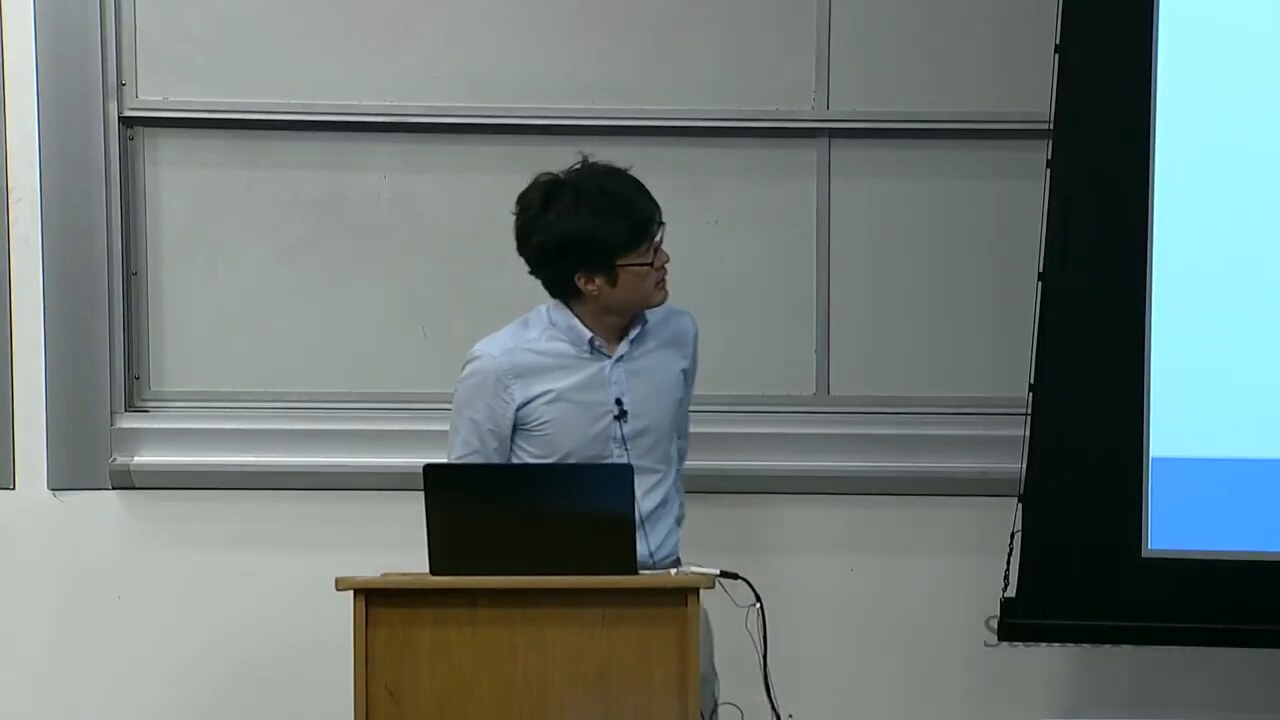
\includegraphics[width=\textwidth]{figures/fig_01.jpg}
\caption{开场回顾：上一节建立的 Kaplan 式经验 Scaling Law 的局限\protect\footnotemark}
\end{figure}
\footnotetext{视频画面时间区间：00:00:15--00:00:45。}

\subsection{为什么需要"更好的"Scaling Laws？}

Kaplan 等人 2020 年的原始 Scaling Law 论文存在几个工程痛点，使其结论在实践中难以直接使用。讲师明确指出了三个关键问题：

\begin{warningbox}{Kaplan Scaling Law 的三个痛点}
\begin{enumerate}
\item \textbf{学习率调度耦合}：Kaplan 实验使用固定的 cosine schedule，每条训练曲线对应一个特定的 LR schedule。要估计 IsoFLOP 曲线上的每一个点，都得重新调 schedule——这在计算上极其昂贵。
\item \textbf{$\alpha$ 与 $\beta$ 难以分离}：Kaplan 拟合的 $L(C) = a \cdot C^{-\alpha}$ 给出了"计算 $\to$ 损失"的整体幂律，但没有显式区分"参数不足"和"数据不足"两种不同的低效来源。
\item \textbf{最优 token/parameter 比例不明}：Kaplan 得出"参数和 token 按相近速率增长"的结论，但这导致 GPT-3 等模型严重\textbf{欠训练}（undertrained）——参数虽多，但训练 token 远不够。
\end{enumerate}
\end{warningbox}

Chinchilla 论文（Hoffmann et al., 2022）的核心贡献，正是用一种更严谨、更可复现的实验设计，给出了\textbf{完全不同的最优 token/parameter 比例}：从 Kaplan 的约 $1.7$ tokens/param 修正到约 $20$ tokens/param。这一发现直接改变了后续所有大模型的训练策略。

\begin{importantbox}{核心结论预告}
给定计算预算 $C$，最优参数量 $N^*$ 和最优 token 数 $D^*$ 应满足：
\[
N^* \propto C^{0.5}, \quad D^* \propto C^{0.5}
\]
即两者按\textbf{相同速率}增长，且 $D^*/N^* \approx 20$。这意味着 Chinchilla 的最优策略是"中等大小但训练充分"，而非 Kaplan 的"大但欠训练"。
\end{importantbox}

\subsection{本节路线图}

\begin{figure}[H]
\centering
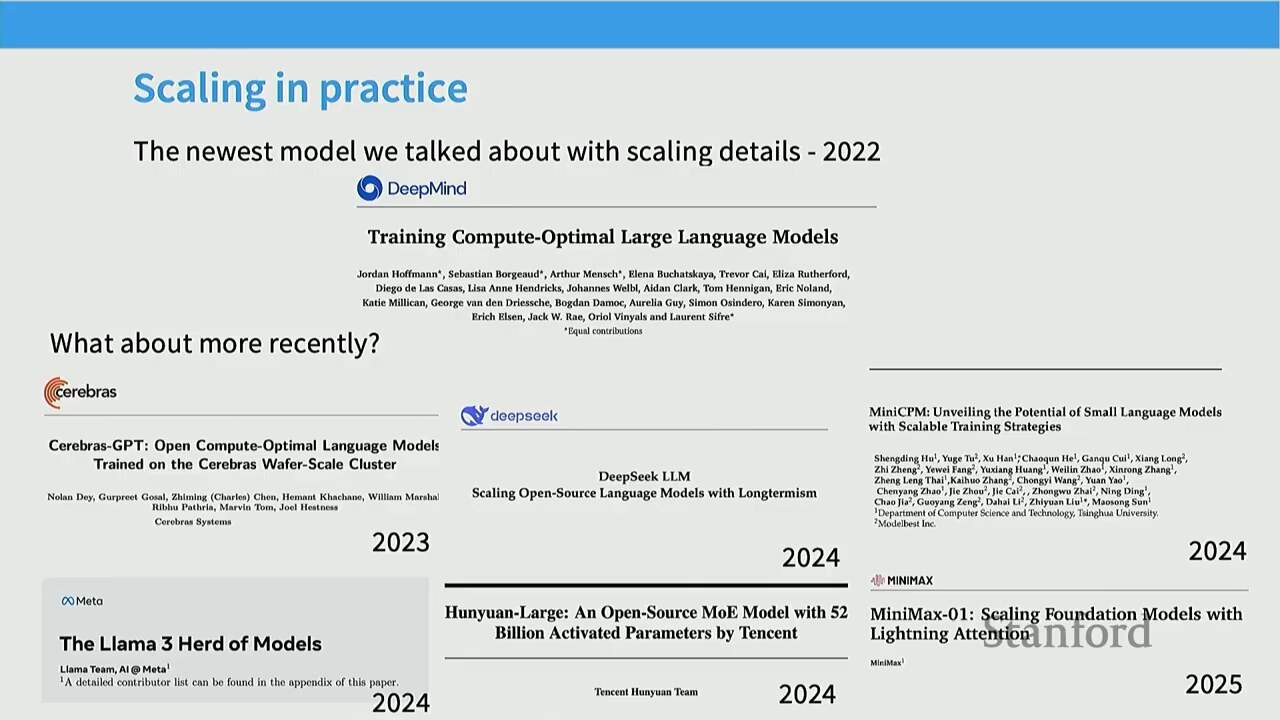
\includegraphics[width=\textwidth]{figures/fig_02.jpg}
\caption{Better scaling laws：本节将系统讲解 Chinchilla 方法论\protect\footnotemark}
\end{figure}
\footnotetext{视频画面时间区间：00:02:00--00:02:30。}

本节分为两大模块：
\begin{itemize}
\item \textbf{模块一（前半段）}：深入 Chinchilla 的方法论——参数化拟合、IsoFLOP 曲线、三种独立估计方法、以及如何解读 Scaling Law 的"含义"。
\item \textbf{模块二（后半段）}：超参数迁移——当模型从 $N_{\text{small}}$ 扩大到 $N_{\text{large}}$ 时，学习率、batch size 等超参数应如何缩放？这是一个在 Kaplan/Chinchilla 框架之外、却同样决定成败的关键问题，最终引出 \textbf{µP（Maximal Update Parametrization）}。
\end{itemize}

\section{Better Scaling Laws：Chinchilla 方法论}

\subsection{参数化损失函数：从单变量到双变量}

\begin{figure}[H]
\centering
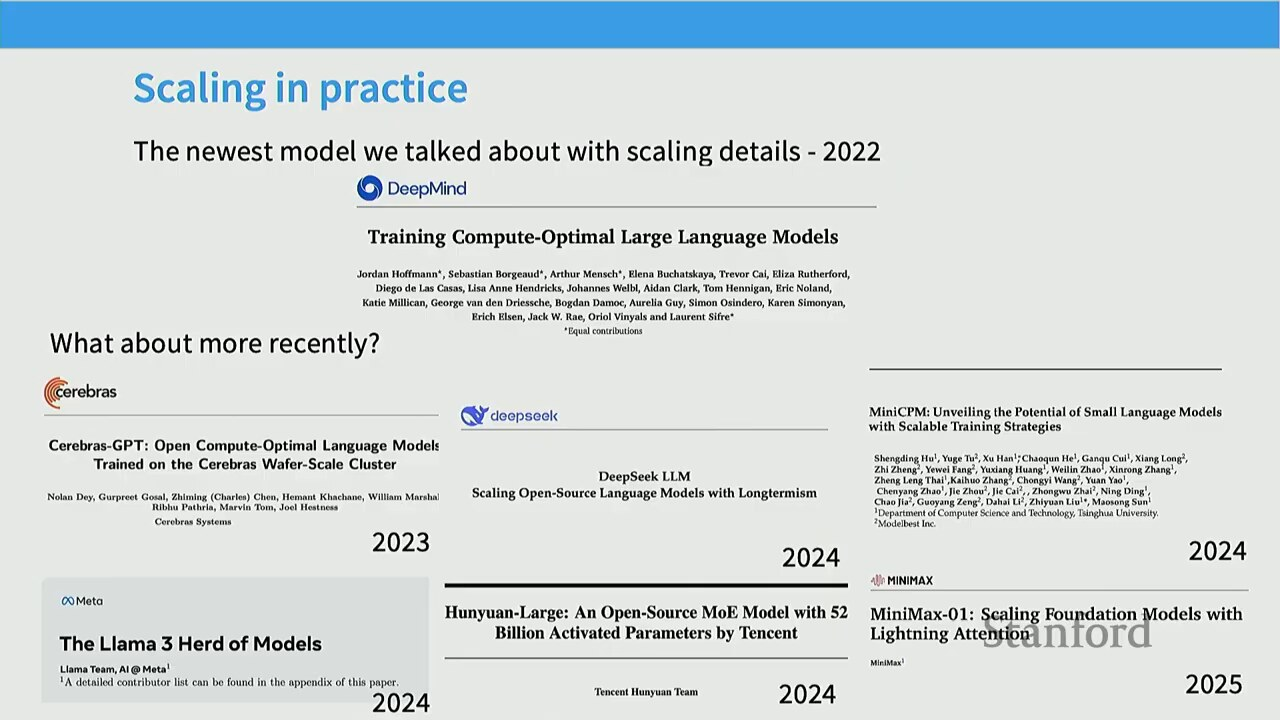
\includegraphics[width=\textwidth]{figures/fig_03.jpg}
\caption{Better scaling laws：双变量损失函数 $L(N, D)$ 的形式\protect\footnotemark}
\end{figure}
\footnotetext{视频画面时间区间：00:03:15--00:03:45。}

Chinchilla 的第一步，是把损失写成参数量 $N$ 和数据量 $D$ 的\textbf{联合}函数，而非 Kaplan 的"通过计算量 $C$ 隐式关联"：

\[
L(N, D) = E + \frac{A}{N^{\alpha_N}} + \frac{B}{D^{\alpha_D}}
\]

\begin{itemize}
\item $E$：\textbf{不可约损失}（irreducible loss），即数据集本身的信息熵下界，无论模型多大、训练多久都无法低于此值。对应自然语言的"真实困惑度"。
\item $A, \alpha_N$：参数不足项，刻画"模型容量不够"导致的损失。
\item $B, \alpha_D$：数据不足项，刻画"见过的 token 不够多"导致的损失。
\item $N$：模型参数量（不含 embedding 时不计词表参数）。
\item $D$：训练 token 数。
\end{itemize}

\begin{knowledgebox}{为何用加法而非乘法？}
加性形式 $E + A/N^{\alpha_N} + B/D^{\alpha_D}$ 隐含假设："参数不足"和"数据不足"是两个\textbf{独立的}低效来源。这并非严格成立——参数不足时，多给数据边际收益也会下降。但加性形式在实验中拟合得很好，且数学上易于求导优化，因此成为事实标准。
\end{knowledgebox}

\subsection{三步法：从损失函数到最优分配}

\begin{figure}[H]
\centering
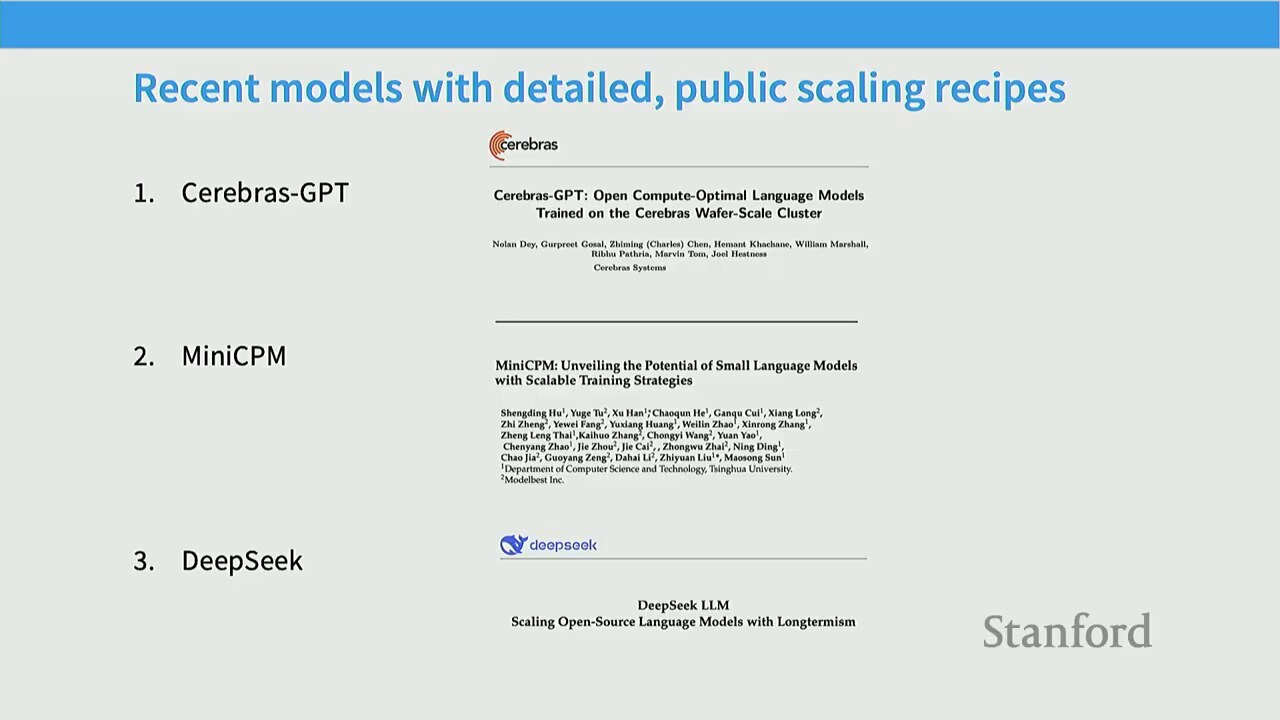
\includegraphics[width=\textwidth]{figures/fig_04.jpg}
\caption{Chinchilla 三步法：参数化拟合 $\to$ 计算约束 $\to$ 求最优 $N^*, D^*$\protect\footnotemark}
\end{figure}
\footnotetext{视频画面时间区间：00:05:45--00:06:15。}

给定损失函数 $L(N, D)$ 后，求"给定计算预算下的最优 $(N^*, D^*)$"是一个标准的约束优化问题：

\begin{importantbox}{最优分配的数学表述}
\textbf{目标}：最小化损失
\[
\min_{N, D} \; L(N, D) = E + \frac{A}{N^{\alpha_N}} + \frac{B}{D^{\alpha_D}}
\]
\textbf{约束}：计算量近似为 $C \approx 6ND$（前向+反向，每参数每 token 共 6 FLOPs）
\[
C = 6 N D
\]

用 Lagrange 乘子法：将 $D = C / (6N)$ 代入，对 $N$ 求导令其为零：
\[
\frac{\partial}{\partial N}\left[ \frac{A}{N^{\alpha_N}} + \frac{B \cdot (6N)^{\alpha_D}}{C^{\alpha_D}} \right] = 0
\]

解得最优 $N^*$ 和 $D^*$ 均与 $C^{0.5}$ 成正比：
\[
N^*(C) = G_N \cdot C^{a}, \quad D^*(C) = G_D \cdot C^{b}
\]
其中经验拟合给出 $a \approx b \approx 0.5$，且 $G_D / G_N \approx 20$。
\end{importantbox}

这意味着最优策略是\textbf{同时放大模型和数据}，而非 Kaplan 建议的"主要放大模型"。两者的核心分歧可以用一个简单的比值刻画：

\[
\frac{D^*}{N^*} \approx 20 \quad \text{(Chinchilla)} \qquad \text{vs.} \qquad \frac{D^*}{N^*} \approx 1.7 \quad \text{(Kaplan)}
\]

\begin{warningbox}{GPT-3 欠训练了多少？}
GPT-3 有 1750 亿参数，按 Kaplan 跑了约 3000 亿 token（$D/N \approx 1.7$）。但按 Chinchilla，1750 亿参数的最优训练量应为 $1750 \times 20 = 3.5$ 万亿 token——GPT-3 的实际训练量\textbf{不到最优值的 10\%}。DeepMind 据此用 700 亿参数的 Chinchilla 模型（训练 1.4 万亿 token）在多数 benchmark 上击败了 GPT-3，用更小的模型、更少总算力，实现了更好的效果。
\end{warningbox}

\subsection{参数化拟合的实验流程}

\begin{figure}[H]
\centering
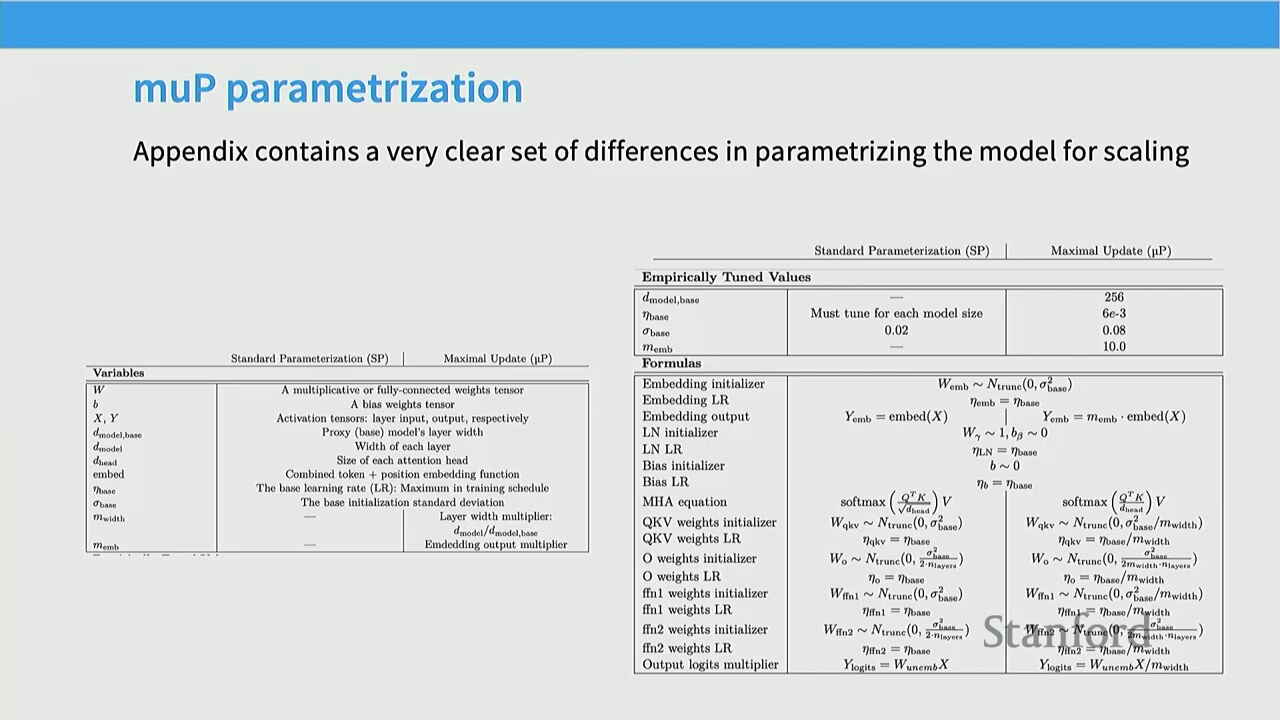
\includegraphics[width=\textwidth]{figures/fig_05.jpg}
\caption{Better scaling laws：参数化拟合的实验设计与数据采集\protect\footnotemark}
\end{figure}
\footnotetext{视频画面时间区间：00:08:45--00:09:15。}

要拟合 $L(N, D)$ 的六个未知数 $(E, A, B, \alpha_N, \alpha_D)$（$E$ 通常单独估），需要在多组 $(N, D)$ 上训练模型，记录最终损失。讲师强调了几个工程细节：

\begin{enumerate}
\item \textbf{学习率调度必须可复现}：每条训练曲线都应使用相同的 LR schedule 策略（如 cosine decay to 10\% of peak），否则不同 $(N, D)$ 的损失不可比。
\item \textbf{训练到收敛}：每个 $(N, D)$ 点都要训到 IsoFLOP 曲线的最低点附近，否则拟合的是"欠训练损失"而非"收敛损失"。
\item \textbf{参数量 $N$ 的定义}：Chinchilla 不计 embedding 参数，因为 embedding 只是查表，不参与核心的前向计算。这与 Kaplan 的统计口径不同，是两者结论差异的部分原因。
\end{enumerate}

\begin{practicebox}{实际拟合代码思路}
\begin{lstlisting}[language=Python, caption={Huber 损失下的 Scaling Law 拟合}]
import numpy as np
from scipy.optimize import curve_fit

def loss_fn(ND, E, A, B, aN, aD):
    N, D = ND
    return E + A / N**aN + B / D**aD

# ND: (N_i, D_i) 训练点; L: 对应最终损失
popt, _ = curve_fit(loss_fn, (N_arr, D_arr), L_arr,
                    p0=[2.0, 100, 100, 0.3, 0.3],
                    bounds=([1, 0, 0, 0, 0], [4, 1e6, 1e6, 1, 1]))
E, A, B, aN, aD = popt
# 最优分配: 给定 C, 求使 L(N, C/(6N)) 最小的 N
\end{lstlisting}
\end{practicebox}

\subsection{IsoFLOP 曲线：可视化最优前沿}

\begin{figure}[H]
\centering
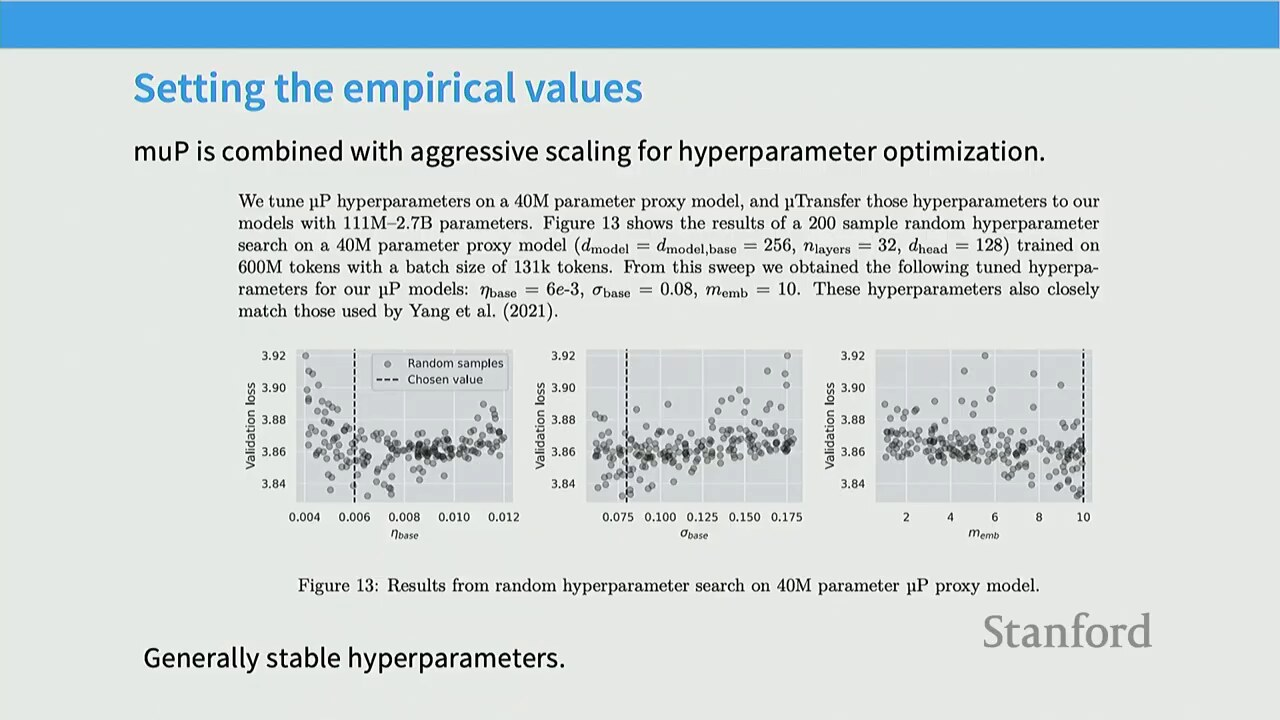
\includegraphics[width=\textwidth]{figures/fig_06.jpg}
\caption{Better scaling laws：IsoFLOP 曲线——固定计算量下，损失随 $N$ 的变化\protect\footnotemark}
\end{figure}
\footnotetext{视频画面时间区间：00:10:30--00:11:00。}

IsoFLOP 曲线是理解 Chinchilla 的关键可视化工具。固定计算量 $C$（即 $6ND = \text{const}$），扫描不同的 $N$（相应地 $D = C/(6N)$），画出损失随 $N$ 的曲线。这条曲线呈 U 形：

\begin{itemize}
\item \textbf{左侧（$N$ 太小）}：模型容量不足，$A/N^{\alpha_N}$ 项主导，损失高。
\item \textbf{右侧（$N$ 太大）}：参数多但 token 少，$B/D^{\alpha_D}$ 项主导（因为 $D = C/(6N)$ 随 $N$ 增大而减小），损失回升。
\item \textbf{谷底}：两条衰退曲线的交点，即该 $C$ 下的最优 $N^*$。
\end{itemize}

\begin{figure}[H]
\centering
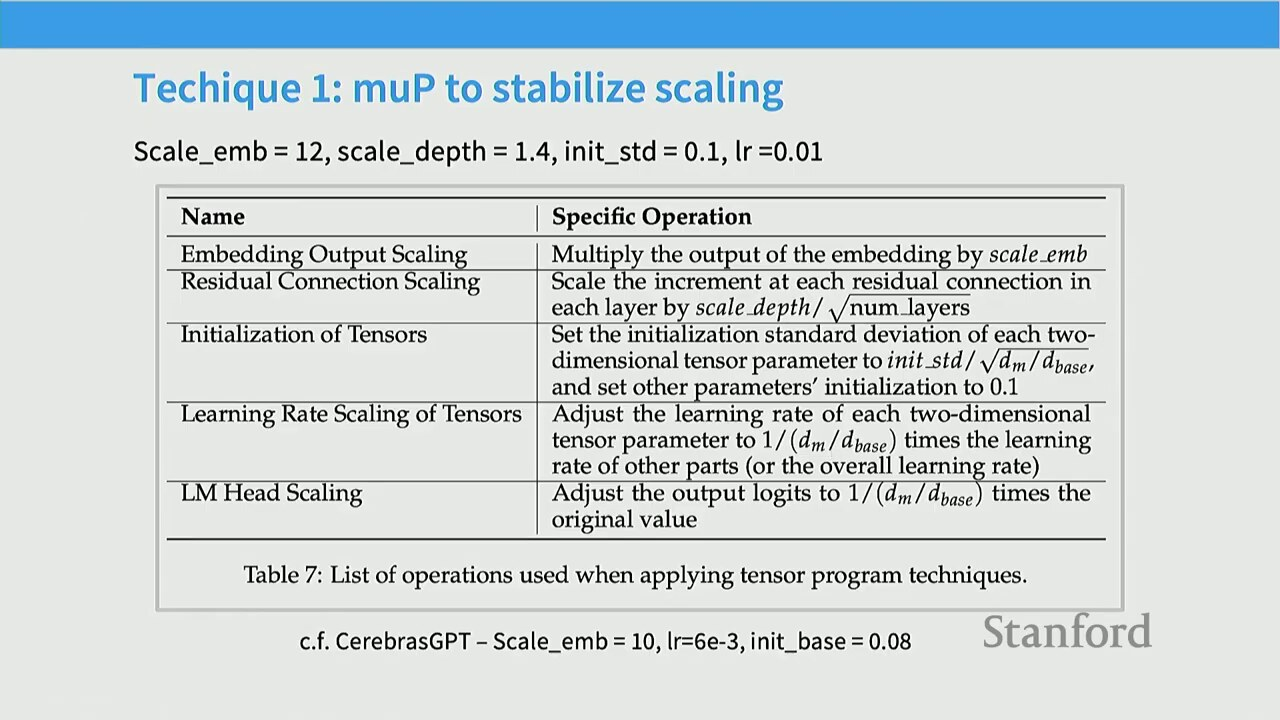
\includegraphics[width=\textwidth]{figures/fig_07.jpg}
\caption{Better scaling laws：等损失曲线族——每条曲线对应一个计算量\protect\footnotemark}
\end{figure}
\footnotetext{视频画面时间区间：00:13:45--00:14:15。}

将不同 $C$ 的 IsoFLOP 谷底点 $(N^*(C), D^*(C))$ 连起来，就得到了\textbf{计算最优前沿}（compute-optimal frontier）。这条前沿在对数-对数坐标下是一条直线，斜率揭示了 $N^*$ 和 $D^*$ 各自随 $C$ 的幂律指数。

\begin{importantbox}{前沿的几何意义}
在 $(\log N, \log D)$ 平面上，等计算量线 $6ND = C$ 是一条斜率为 $-1$ 的直线。最优前沿是这些直线与等损失椭圆的切点轨迹。前沿的斜率若为正且小于 $-1$ 的绝对值（实际约为 $-0$ 附近，即接近水平），意味着 $N$ 和 $D$ 应\textbf{等比例}增长。这正是 Chinchilla $a \approx b \approx 0.5$ 的几何直觉。
\end{importantbox}

\subsection{完整损失公式的拟合结果}

\begin{figure}[H]
\centering
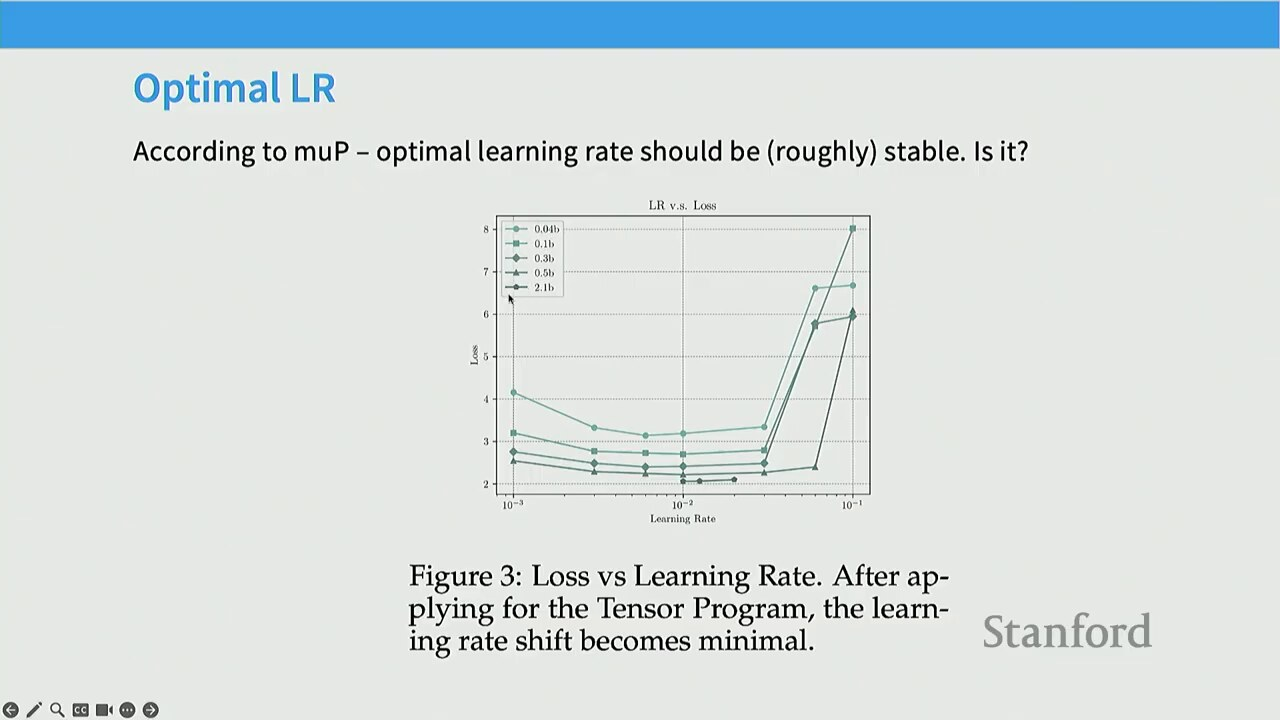
\includegraphics[width=\textwidth]{figures/fig_08.jpg}
\caption{Better scaling laws：完整参数化损失 $L(N,D) = E + A/N^{\alpha} + B/D^{\beta}$\protect\footnotemark}
\end{figure}
\footnotetext{视频画面时间区间：00:17:30--00:18:00。}

Chinchilla 论文给出的拟合参数（数值因实现而略有差异，以下为典型量级）：

\begin{tabular}{p{3cm}p{4cm}p{6cm}}
\toprule
\textbf{参数} & \textbf{典型值} & \textbf{含义} \\
\midrule
$E$ & $\approx 1.69$（nats） & 不可约损失，对应数据集的信息熵下界 \\
$A$ & $\approx 406$ & 参数不足项的系数 \\
$B$ & $\approx 410$ & 数据不足项的系数 \\
$\alpha_N$ & $\approx 0.34$ & 参数不足的幂律指数 \\
$\alpha_D$ & $\approx 0.28$ & 数据不足的幂律指数 \\
\bottomrule
\end{tabular}

\vspace{0.3cm}

注意 $\alpha_N \approx \alpha_D$（都在 $0.3$ 附近），这是 $N^*$ 和 $D^*$ 按相同速率增长（$C^{0.5}$）的数学根源。如果 $\alpha_N > \alpha_D$，则参数不足的损失下降更快，最优策略会偏向"小模型多数据"；反之亦然。

\begin{knowledgebox}{$\alpha$ 值的敏感性分析}
最优分配 $N^*(C)$ 的指数 $a$ 不仅取决于 $\alpha_N, \alpha_D$，还取决于两者之比。具体地：
\[
a = \frac{\alpha_D}{\alpha_N + \alpha_D}
\]
若 $\alpha_N = \alpha_D$，则 $a = 0.5$。Chinchilla 的拟合给出 $a \approx 0.46$–$0.5$，接近理论值。但 $\alpha$ 的估计本身有噪声——$\pm 0.02$ 的波动就能让 $a$ 在 $0.45$–$0.55$ 间漂移。这也是为什么 Chinchilla 用\textbf{三种独立方法}交叉验证。
\end{knowledgebox}

\subsection{学习率调度的影响}

\begin{figure}[H]
\centering
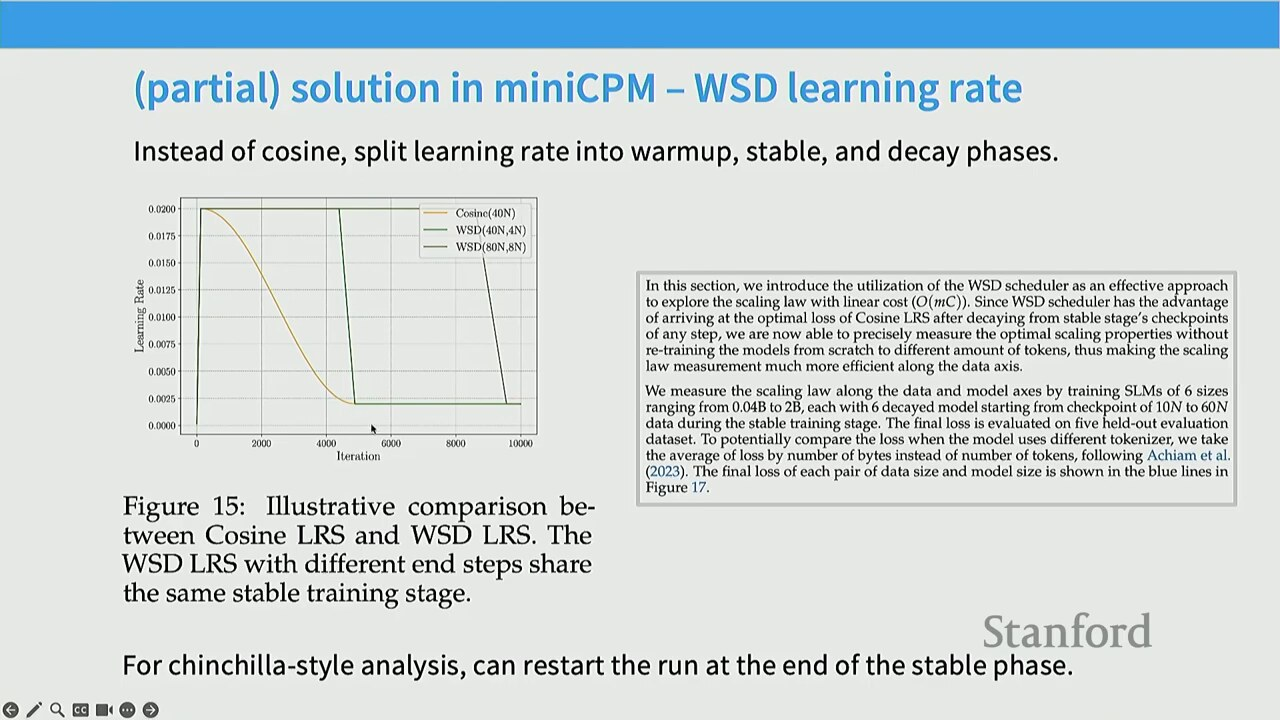
\includegraphics[width=\textwidth]{figures/fig_09.jpg}
\caption{Better scaling laws：学习率调度对损失曲线的影响\protect\footnotemark}
\end{figure}
\footnotetext{视频画面时间区间：00:21:15--00:21:45。}

讲师特别强调了学习率调度的复杂性。Kaplan 论文为每条曲线单独调 LR schedule，导致 IsoFLOP 曲线的不同点对应不同的训练动态，可比性存疑。Chinchilla 的改进是：

\begin{itemize}
\item \textbf{统一的 schedule 策略}：所有训练运行使用相同的 cosine decay 形式（峰值 LR 因模型而异，但 decay 比例固定）。
\item \textbf{训练到充分收敛}：每个 $(N, D)$ 点都训练到 IsoFLOP 曲线的最低点，而非固定 epoch 数。
\end{itemize}

\begin{warningbox}{"充分收敛"的陷阱}
判断"充分收敛"本身需要经验。如果训练步数不够，拟合出的 $\alpha$ 会偏小（因为损失还在下降，没有触底）。讲师提到一个实用技巧：用 cosine schedule 的"冷却"阶段（cool down）反复训练，取损失的\textbf{下包络}（lower envelope）作为收敛损失的估计。这样可以部分缓解"何时算收敛"的不确定性。
\end{warningbox}

\subsection{Compute-Optimal 前沿}

\begin{figure}[H]
\centering
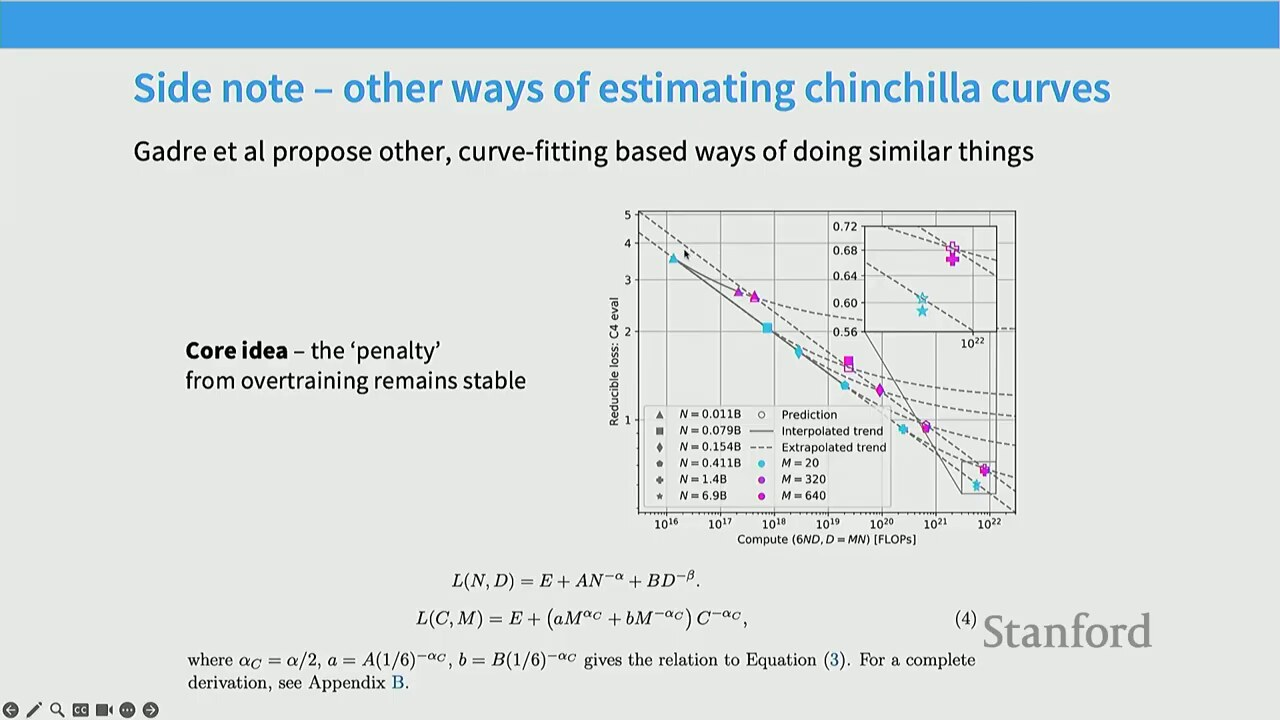
\includegraphics[width=\textwidth]{figures/fig_10.jpg}
\caption{Better scaling laws：Compute-Optimal 前沿——最优 $(N^*, D^*)$ 随 $C$ 的轨迹\protect\footnotemark}
\end{figure}
\footnotetext{视频画面时间区间：00:25:00--00:25:30。}

将所有 IsoFLOP 曲线的谷底连接起来，得到一条在 $(\log N, \log D)$ 平面上的直线。这条直线的斜率接近 $1$（即 $N^* \propto D^*$），截距给出 $D^*/N^* \approx 20$。

\begin{figure}[H]
\centering
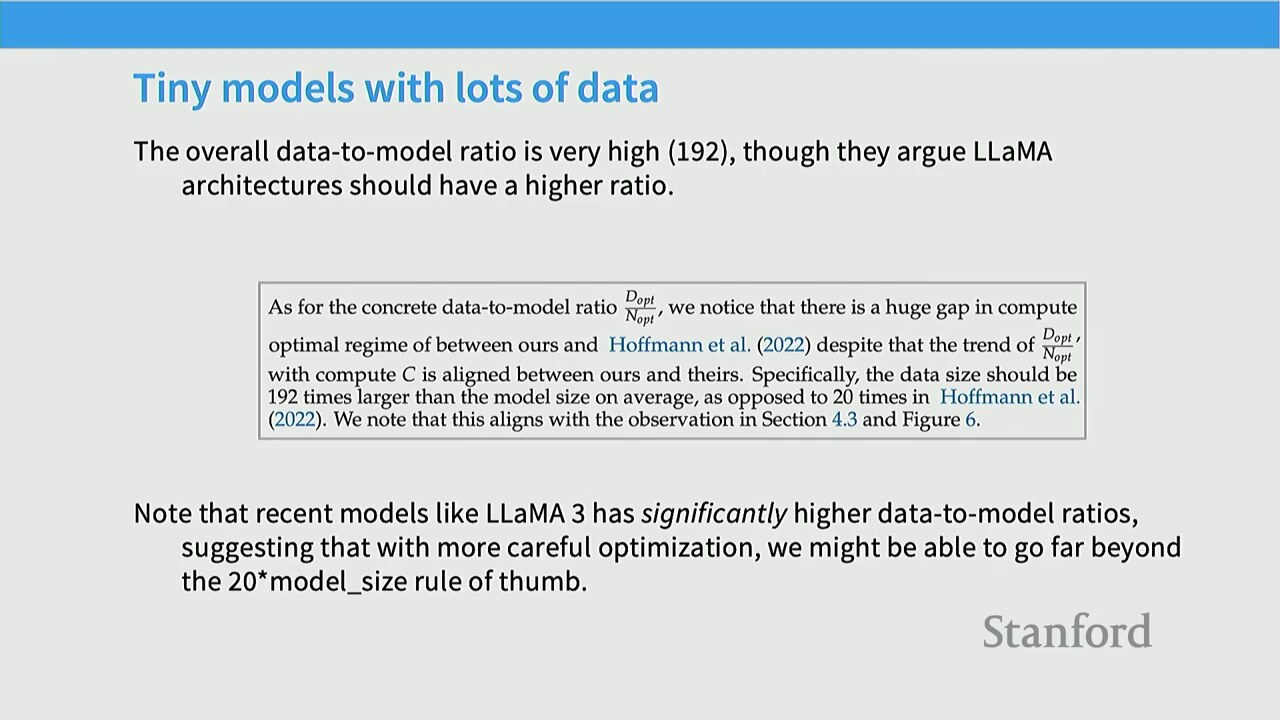
\includegraphics[width=\textwidth]{figures/fig_11.jpg}
\caption{Better scaling laws：完整 loss 拟合的残差与置信区间\protect\footnotemark}
\end{figure}
\footnotetext{视频画面时间区间：00:27:30--00:28:00。}

讲师展示了拟合的残差图，强调拟合在中间计算量区间（$10^{18}$--$10^{21}$ FLOPs）非常准确，但在极小或极大区间外推时置信区间会变宽。这意味着：

\begin{importantbox}{Scaling Law 的外推风险}
从 $10^{21}$ FLOPs 的实验拟合出的指数，外推到 $10^{25}$ FLOPs（如 GPT-4 级别）时存在系统性误差风险。实际上，后来的研究（如 Llama 3、DeepSeek）发现，在极大计算量下，最优 $D/N$ 比例可能进一步上升（"过度训练"趋势），这与 Chinchilla 的 $C^{0.5}$ 外推不完全一致。本节后半段将讨论这种偏离。
\end{importantbox}

\subsection{Chinchilla 的三种独立方法}

\begin{figure}[H]
\centering
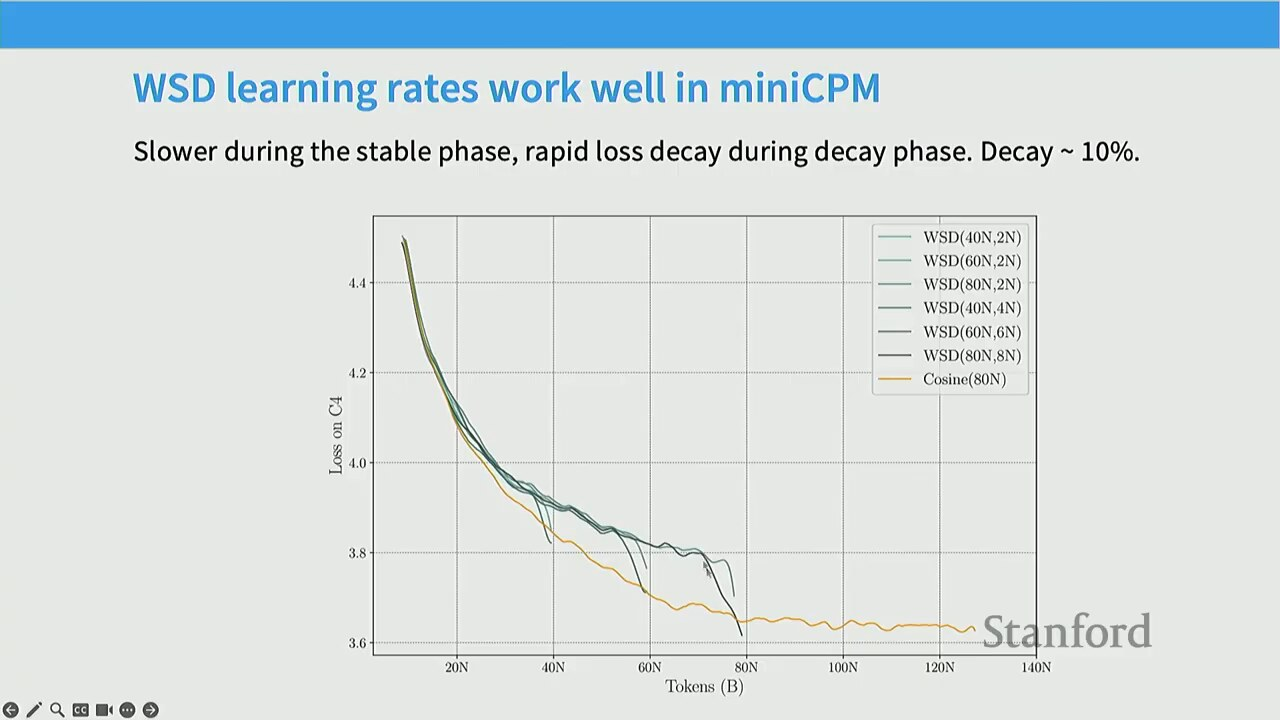
\includegraphics[width=\textwidth]{figures/fig_12.jpg}
\caption{Better scaling laws：Chinchilla 三种独立方法交叉验证\protect\footnotemark}
\end{figure}
\footnotetext{视频画面时间区间：00:31:15--00:31:45。}

为增强结论的稳健性，Chinchilla 论文使用了三种\textbf{方法论上独立}的估计方法，交叉验证 $N^*(C)$ 和 $D^*(C)$：

\begin{enumerate}
\item \textbf{方法一：参数化拟合（Approach 1）}。直接拟合 $L(N, D) = E + A/N^{\alpha_N} + B/D^{\alpha_D}$，然后解析求最优。这是前面讲的标准流程。

\item \textbf{方法二：固定 $N$，扫描 $D$（Approach 2 -- IsoFLOP）}。对每个固定的 $N$，训练多个不同 $D$ 的模型，找到使该 $N$ 下损失最低的 $D$。这给出 IsoFLOP 曲线族的谷底，\textbf{不依赖}参数化假设。

\item \textbf{方法三：固定计算量，扫描 $(N, D)$ 组合（Approach 3）}。对每个固定的 $C$，训练多组 $(N, D)$（满足 $6ND = C$），直接找损失最低的组合。这是最直接的"实验测量"，无需任何参数化模型。
\end{enumerate}

\begin{figure}[H]
\centering
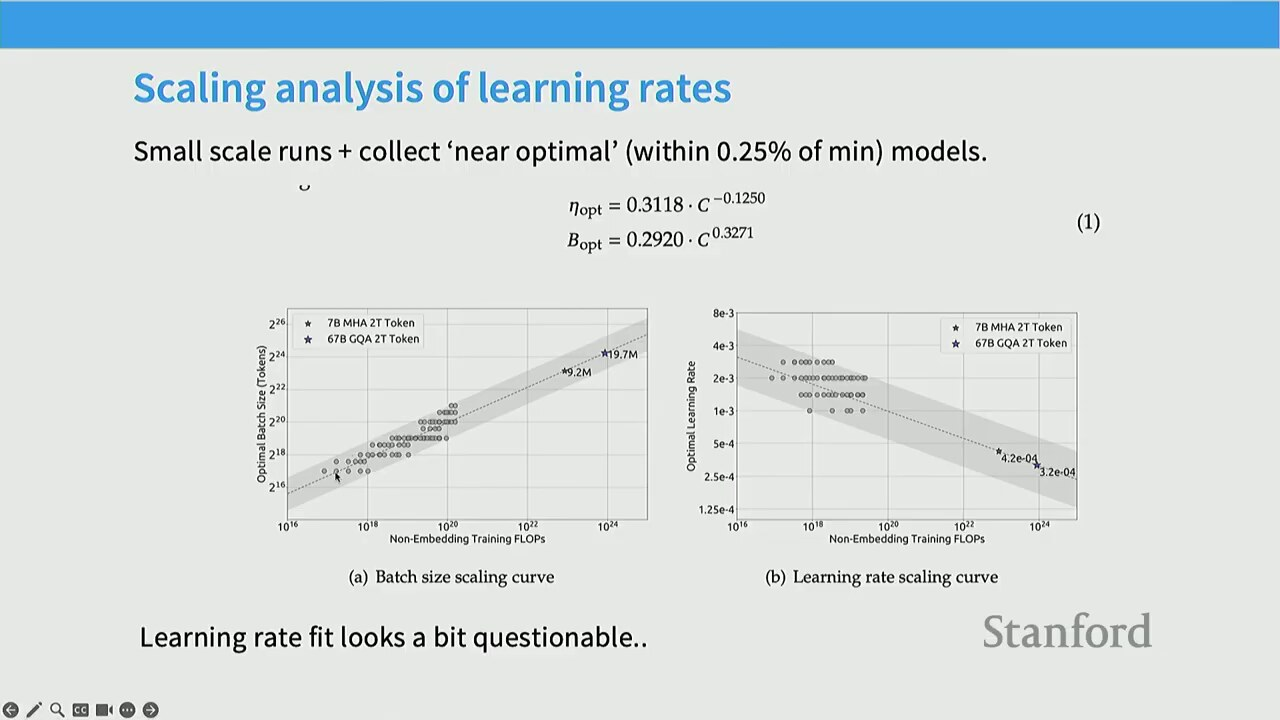
\includegraphics[width=\textwidth]{figures/fig_13.jpg}
\caption{Better scaling laws：三种方法的 IsoFLOP 曲线对比与一致性检验\protect\footnotemark}
\end{figure}
\footnotetext{视频画面时间区间：00:35:00--00:35:30。}

\begin{practicebox}{三种方法的一致性}
三种方法独立得到的 $N^*(C) \propto C^{0.5}$ 和 $D^*(C) \propto C^{0.5}$ 几乎完全一致。这种\textbf{方法论交叉验证}是 Chinchilla 结论可信的关键——单一方法的偏差被另外两种方法修正。讲师特别指出，方法二和方法三因为不依赖参数化假设，在计算量极大区间（$> 10^{22}$ FLOPs）的估计可能比方法一更可靠，因为参数化模型在那里的外推误差最大。
\end{practicebox}

\section{Scaling Laws 的真正含义}

\subsection{它们在统计什么？}

\begin{figure}[H]
\centering
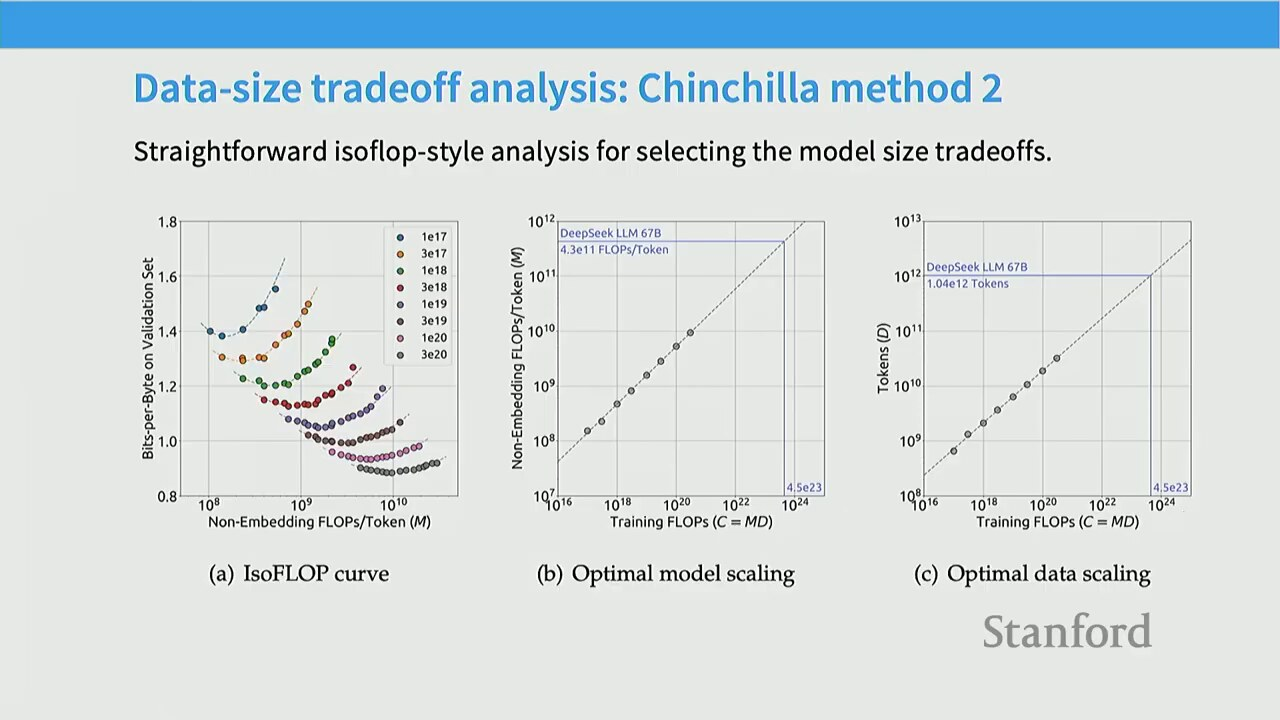
\includegraphics[width=\textwidth]{figures/fig_14.jpg}
\caption{Scaling laws: what they mean——Scaling Law 是关于数据分布的统计陈述\protect\footnotemark}
\end{figure}
\footnotetext{视频画面时间区间：00:37:30--00:38:00。}

讲师在这一节提出了一个深刻的方法论问题：Scaling Law 到底在刻画什么？他的核心论点是：

\begin{importantbox}{Scaling Law 的本质}
Scaling Laws 是关于\textbf{特定数据分布}的统计陈述。它们回答的问题是："在分布 $\mathcal{D}$ 上，给定 $(N, D)$，模型的期望损失是多少？" 损失 $L$ 是模型在分布 $\mathcal{D}$ 上的交叉熵，即：
\[
L(N, D) = -\mathbb{E}_{x \sim \mathcal{D}}\left[\log p_{\theta}(x)\right]
\]

\begin{itemize}
\item $p_{\theta}(x)$：模型对样本 $x$ 的预测概率
\item $\mathcal{D}$：目标数据分布（通常是训练数据所代表的互联网文本分布）
\item $L$：在该分布上的平均负对数似然
\end{itemize}
\end{importantbox}

这意味着 Scaling Law 的一切结论——最优 $N^*, D^*$、幂律指数 $\alpha$——都\textbf{依赖于 $\mathcal{D}$}。换一个数据分布（如代码 vs. 自然语言，或高质量过滤数据 vs. 原始 Common Crawl），拟合出的参数会完全不同。

\subsection{数据质量改变 Scaling Law}

\begin{warningbox}{数据质量是最强的"调节旋钮"}
如果用高质量、经过清洗和去重的数据训练，相同 $(N, D)$ 下的损失会显著低于用原始网页爬取数据。这意味着：
\begin{itemize}
\item 高质量数据的 $E$（不可约损失）更低——因为数据"更可预测"。
\item 高质量数据的 $\alpha$ 也可能更大——损失下降更快，因为每多一个 token 的边际信息量更高。
\item 结果：最优 $D^*$ 可能\textbf{变小}——你不需要那么多 token 就能达到相同损失。
\end{itemize}
这正是为什么 Llama 3 等模型即使训练 token 数远超 Chinchilla 最优值，性能仍在提升——它们用的是更高质量、更高效的数据。
\end{warningbox}

\subsection{下游任务 vs. 训练损失}

Scaling Law 通常拟合的是\textbf{训练损失}（交叉熵）。但实际关心的往往是\textbf{下游任务}表现（如 MMLU、HumanEval）。两者之间存在复杂关系：

\begin{itemize}
\item \textbf{线性区}：在大多数任务上，下游准确率与训练损失近似对数线性相关——损失每降低固定量，下游准确率提升固定比例。这就是著名的"log-linear scaling"。
\item \textbf{相变区}：某些任务（如 in-context learning、链式推理）存在\textbf{涌现现象}——损失降到某个阈值前，下游表现几乎为零；越过阈值后突然跃升。这种非线性使得从训练损失外推下游表现变得不可靠。
\end{itemize}

\begin{knowledgebox}{涌现能力的争议}
Schaeffer et al. (2023) 指出，许多"涌现"可能只是评价指标的非线性（如 exact-match 从 0 跳到 1）造成的假象——改用连续指标（如 Brier score）后，相变变成平滑过渡。但无论如何，从训练损失预测下游表现需要谨慎，不能简单外推。
\end{knowledgebox}

\subsection{Scaling Law 的适用边界}

\begin{figure}[H]
\centering
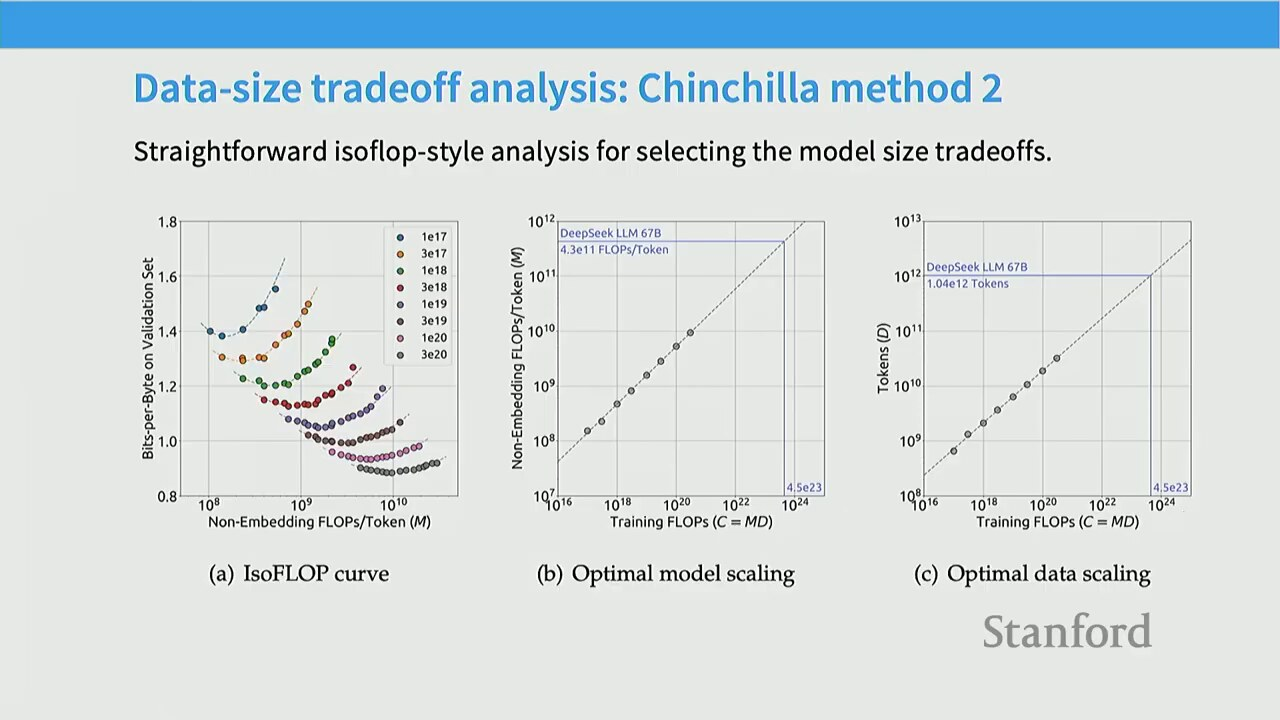
\includegraphics[width=\textwidth]{figures/fig_14.jpg}
\caption{Scaling laws 的适用边界：何时外推会失效\protect\footnotemark}
\end{figure}
\footnotetext{视频画面时间区间：00:39:00--00:39:30。}

讲师总结了几种 Scaling Law 外推失效的典型情形：

\begin{enumerate}
\item \textbf{数据耗尽}：Chinchilla 假设数据无限。但当 $D^*$ 超过高质量数据的总量时（如互联网去重后约 10--20 万亿 token），无法继续按 $D^* \propto C^{0.5}$ 增长，模型被迫"数据受限"。
\item \textbf{架构变更}：Scaling Law 是针对特定架构（如 dense Transformer）拟合的。换成 MoE、稀疏注意力、或全新架构，幂律指数会变。
\item \textbf{任务特异性}：训练损失的外推对通用任务较准，但对特定能力（如数学推理、代码生成）的外推误差大。
\end{enumerate}

\section{超参数缩放：一个被忽视的问题}

\subsection{问题陈述：从 $N_{\text{small}}$ 到 $N_{\text{large}}$}

\begin{figure}[H]
\centering
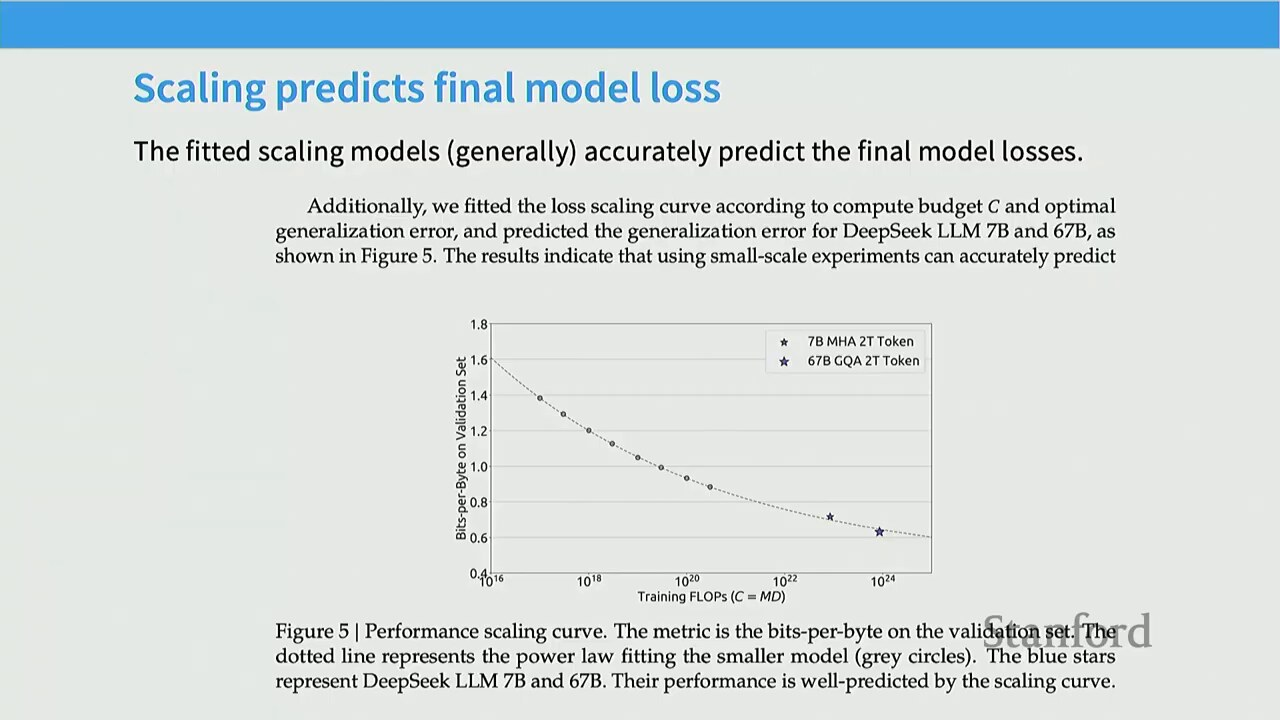
\includegraphics[width=\textwidth]{figures/fig_15.jpg}
\caption{How should we scale learning rate and batch size?——超参数迁移的核心问题\protect\footnotemark}
\end{figure}
\footnotetext{视频画面时间区间：00:40:00--00:40:30。}

至此，Chinchilla 回答了"给定计算预算，最优 $(N, D)$ 是多少"。但还有一个关键的工程问题没有回答：\textbf{当模型从 $N_{\text{small}}$ 扩大到 $N_{\text{large}}$ 时，超参数应如何缩放？}

具体而言，假设你在小模型上通过网格搜索找到了最优：
\begin{itemize}
\item 峰值学习率 $\eta_{\text{small}}^*$
\item Batch size $B_{\text{small}}^*$
\item 权重初始化的标准差 $\sigma_{\text{small}}^*$
\item 各种正则化系数
\end{itemize}

现在你要训练一个 100 倍大的模型。\textbf{这些超参数应该怎么变？} 直接复制显然不行——大模型用小模型的学习率会发散；用大 batch size 则梯度噪声结构不同。

\begin{importantbox}{为什么不能直接网格搜索？}
在大模型上网格搜索学习率，每次试错都烧几十万美元。如果有一个理论框架能从小模型的超参数\textbf{推导}出大模型的超参数，就能省下巨额成本。这正是 µP（Maximal Update Parametrization）要解决的问题。
\end{importantbox}

\subsection{宽度缩放：以宽度 $m$ 为桥梁}

\begin{figure}[H]
\centering
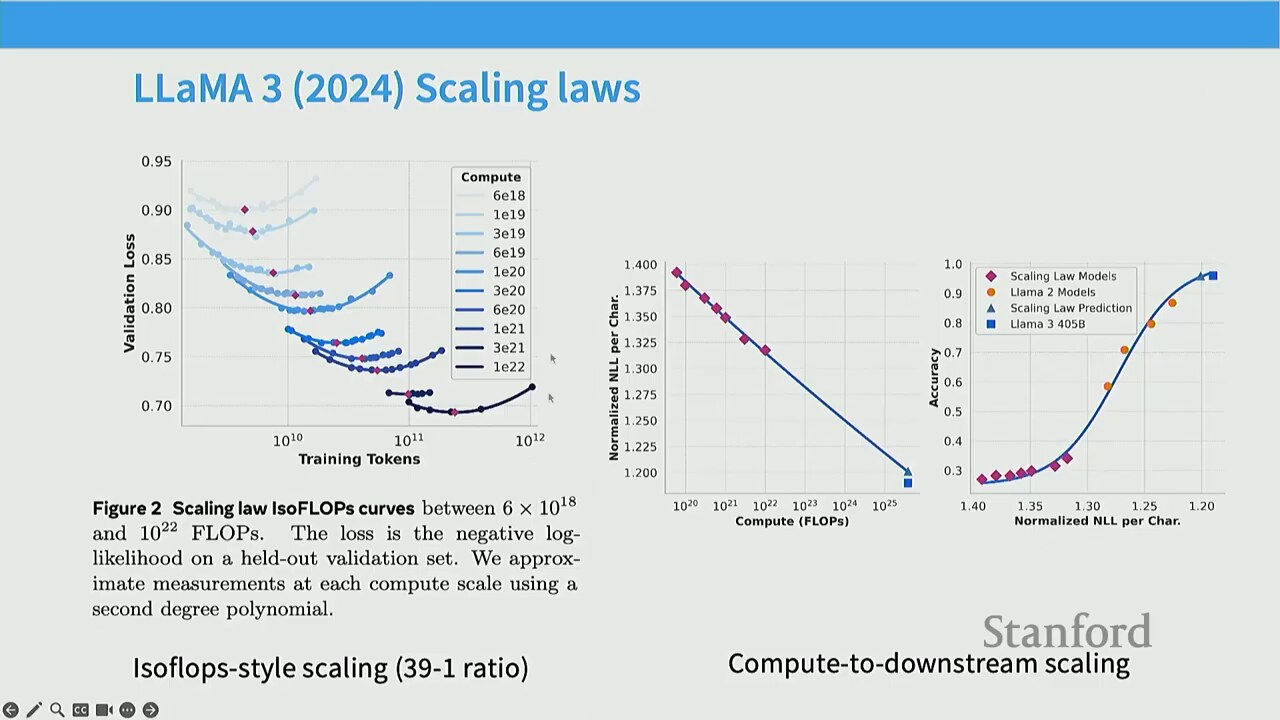
\includegraphics[width=\textwidth]{figures/fig_16.jpg}
\caption{超参数迁移：以网络宽度 $m$ 为缩放桥梁\protect\footnotemark}
\end{figure}
\footnotetext{视频画面时间区间：00:42:30--00:43:00。}

讲师将问题简化为\textbf{宽度缩放}（width scaling）：固定网络深度，把宽度（隐藏层维度）从 $d$ 扩大到 $m \cdot d$，其中 $m$ 是宽度缩放因子。分析激活值、梯度、权重更新如何随 $m$ 变化。

\begin{figure}[H]
\centering
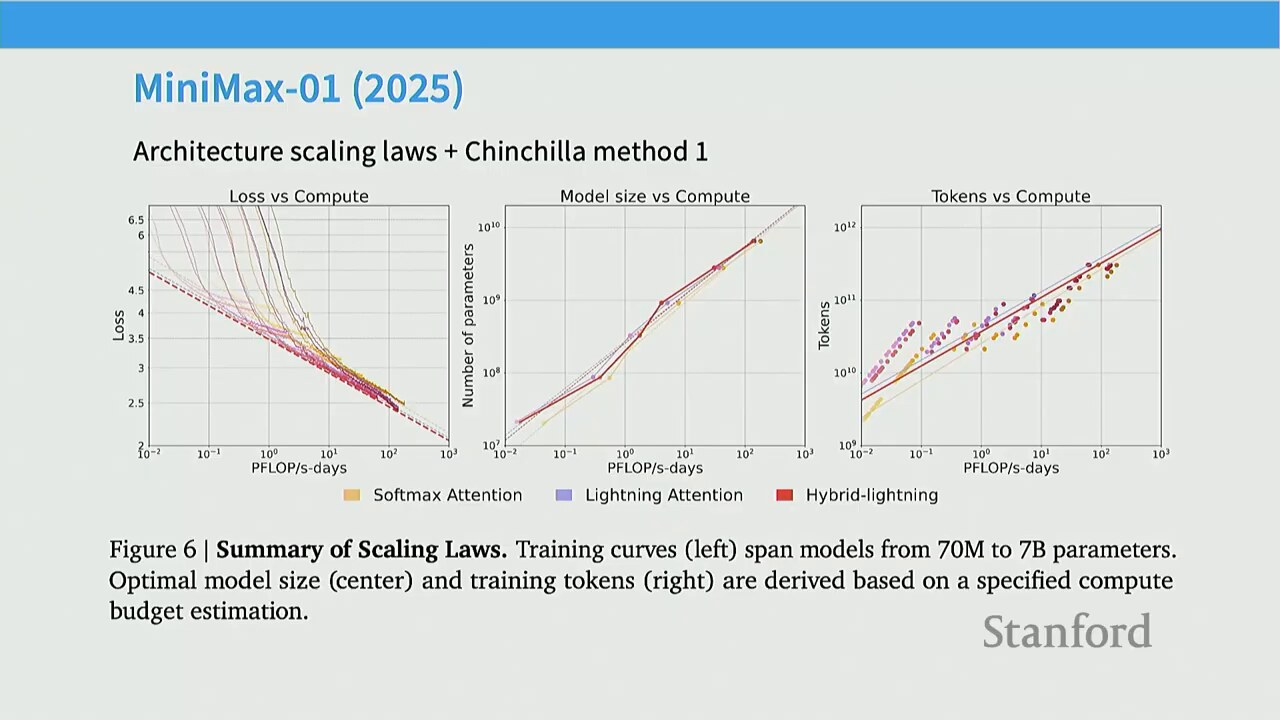
\includegraphics[width=\textwidth]{figures/fig_17.jpg}
\caption{Hyperparameter transfer: experimental setup——宽度扫描实验设计\protect\footnotemark}
\end{figure}
\footnotetext{视频画面时间区间：00:45:00--00:45:30。}

为什么要选宽度而非深度？因为：
\begin{itemize}
\item 宽度增加是最常见的扩缩方向（GPT 系列从 $d=768$ 到 $d=12288$）。
\item 宽度缩放的数学分析比深度缩放更干净——每层的统计性质可以直接对 $m$ 求期望。
\item 宽度足够大时，网络的某些性质会"饱和"（收敛到无限宽极限），这正是 Neural Tangent Kernel 和 µP 的理论基础。
\end{itemize}

\subsection{实验观察：学习率应如何缩放}

\begin{figure}[H]
\centering
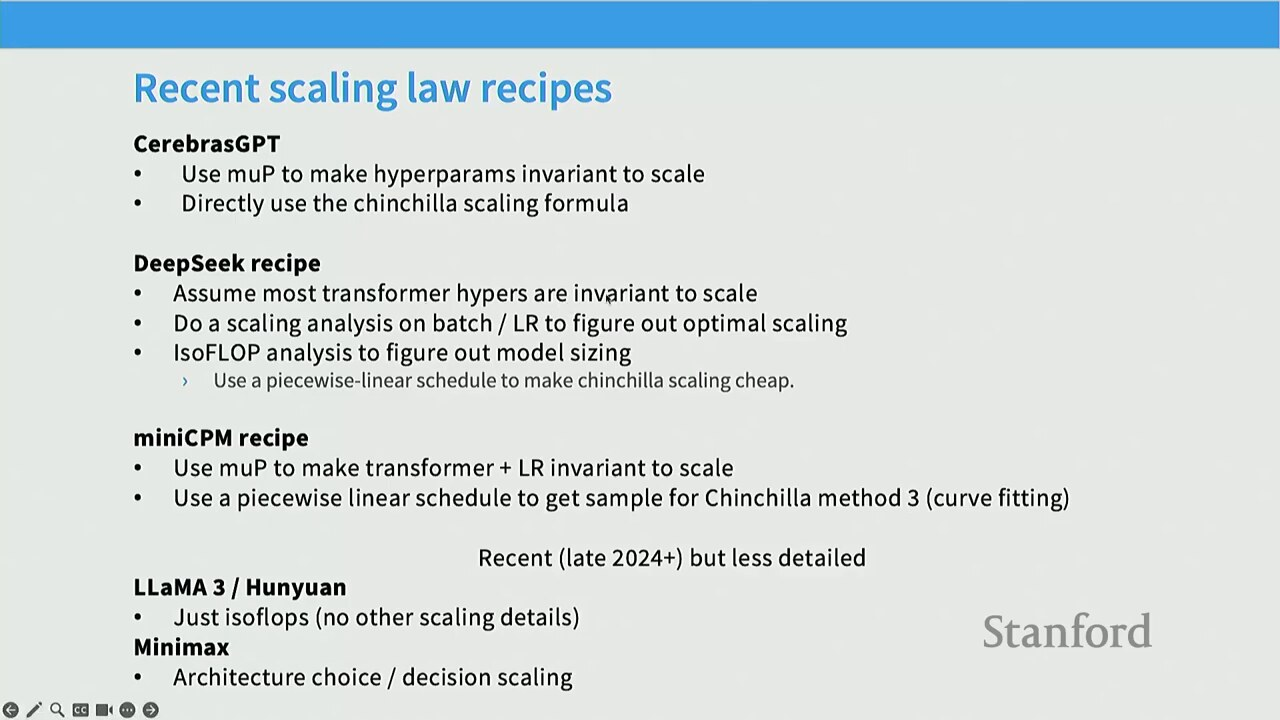
\includegraphics[width=\textwidth]{figures/fig_18.jpg}
\caption{Hyperparameter transfer：不同宽度下最优学习率的扫描结果\protect\footnotemark}
\end{figure}
\footnotetext{视频画面时间区间：00:47:30--00:48:00。}

讲师展示了实验结果：对每个宽度 $m$，扫描学习率，找到使训练损失最低的 $\eta^*(m)$。关键观察是：

\[
\eta^*(m) \propto \frac{1}{m}
\]

\begin{figure}[H]
\centering
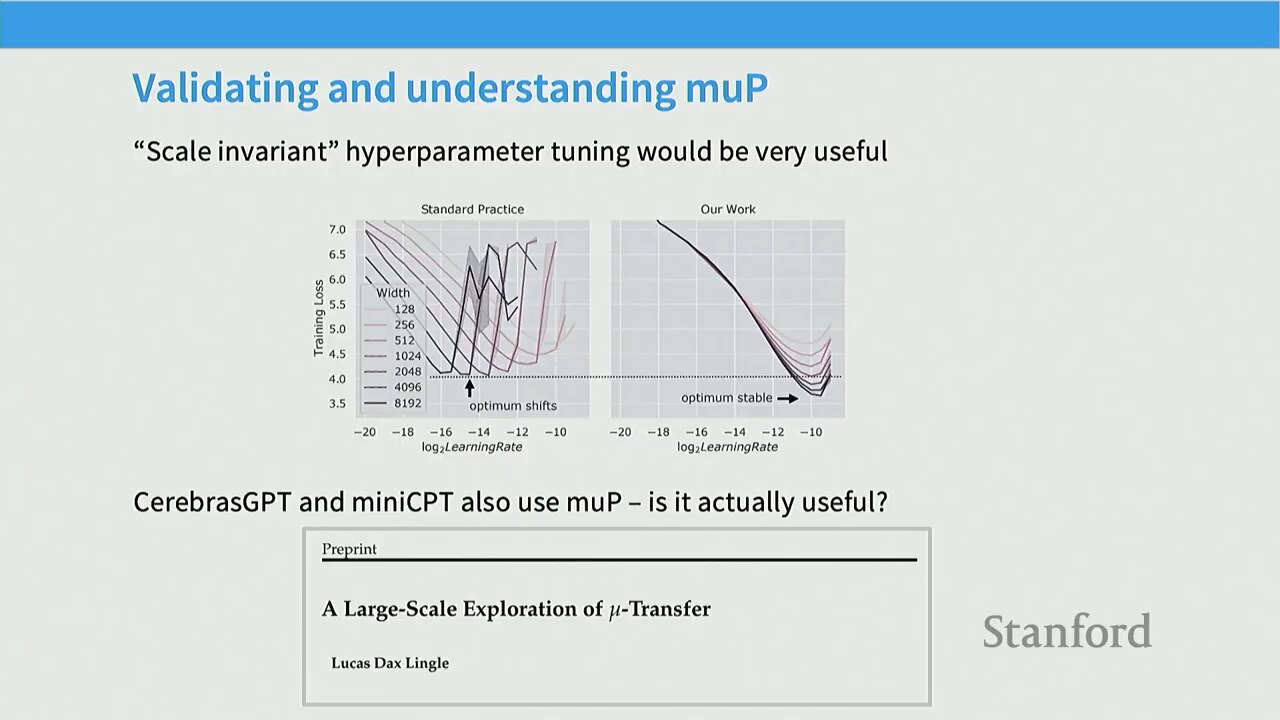
\includegraphics[width=\textwidth]{figures/fig_19.jpg}
\caption{Hyperparameter transfer：学习率缩放公式 $\eta^* \propto 1/m$ 的实验验证\protect\footnotemark}
\end{figure}
\footnotetext{视频画面时间区间：00:50:00--00:50:30。}

即\textbf{最优学习率与宽度成反比}。宽度翻倍，学习率减半。这与朴素的"大模型用大学习率"直觉相反。

\begin{warningbox}{朴素直觉为何失效？}
直觉上，参数越多，梯度方向越可靠，应该能用更大学习率。但实验显示相反。原因在于：宽度增加时，每个神经元接收的输入增多，梯度的\textbf{方差}也随之增大（因为更多独立信号的叠加）。如果不调小学习率，单步更新的"幅度"会爆炸，导致训练发散。µP 的推导正是要精确量化这种方差增长。
\end{warningbox}

\subsection{验证：从小模型迁移到大模型}

\begin{figure}[H]
\centering
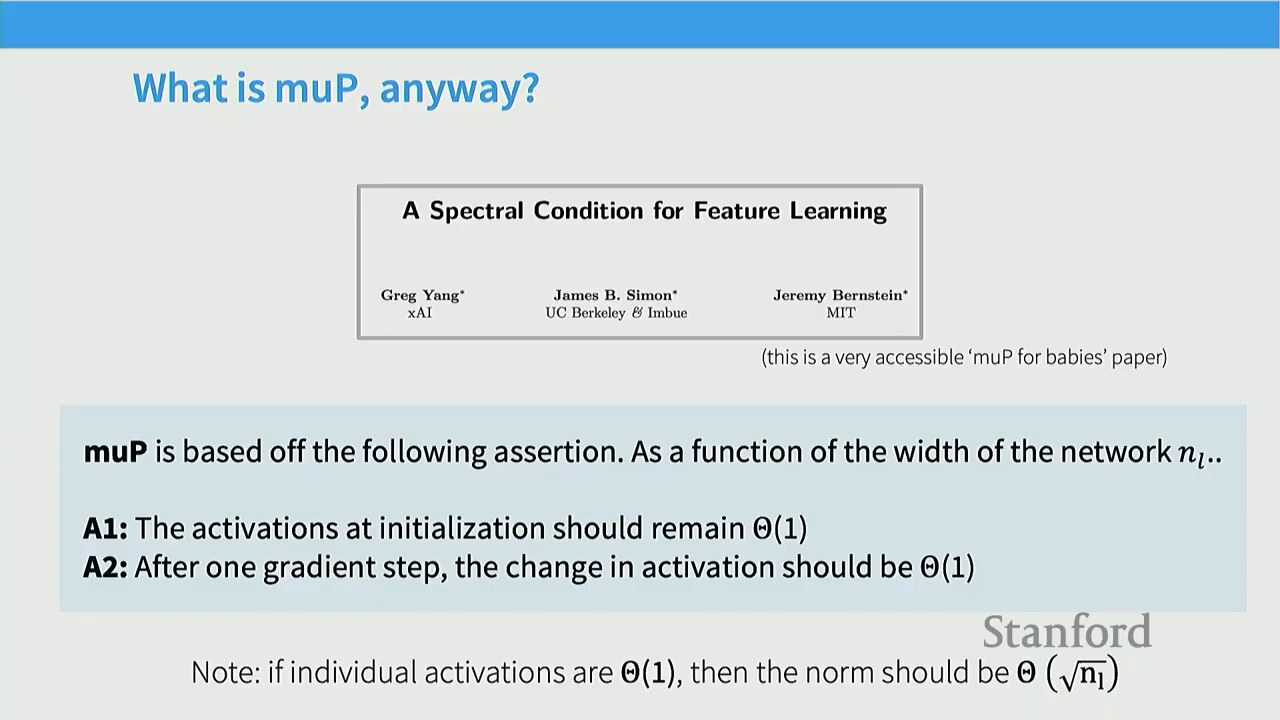
\includegraphics[width=\textwidth]{figures/fig_20.jpg}
\caption{Hyperparameter transfer：从小模型迁移到大模型的验证结果\protect\footnotemark}
\end{figure}
\footnotetext{视频画面时间区间：00:52:30--00:53:00。}

讲师展示了关键验证：在小模型（如 $d=128$）上找到最优学习率 $\eta^*_{\text{small}}$，然后按 $\eta^*_{\text{large}} = \eta^*_{\text{small}} / m$ 推算大模型（如 $d=4096$，$m=32$）的学习率。结果显示，这个推算值与大模型上独立网格搜索的最优值\textbf{高度一致}——迁移是有效的。

\begin{practicebox}{工程收益}
µP 的迁移意味着：你只需要在小模型上做一次昂贵的超参数搜索，然后\textbf{免费}获得所有大模型的超参数。对于一个要训 10 个不同规模模型的团队，这是数量级的成本节省。这正是 µP 在工业界（如 Anthropic、Meta）被广泛采用的原因。
\end{practicebox}

\section{Maximal Update Parametrization (µP)}

\subsection{动机：从经验观察到理论框架}

\begin{figure}[H]
\centering
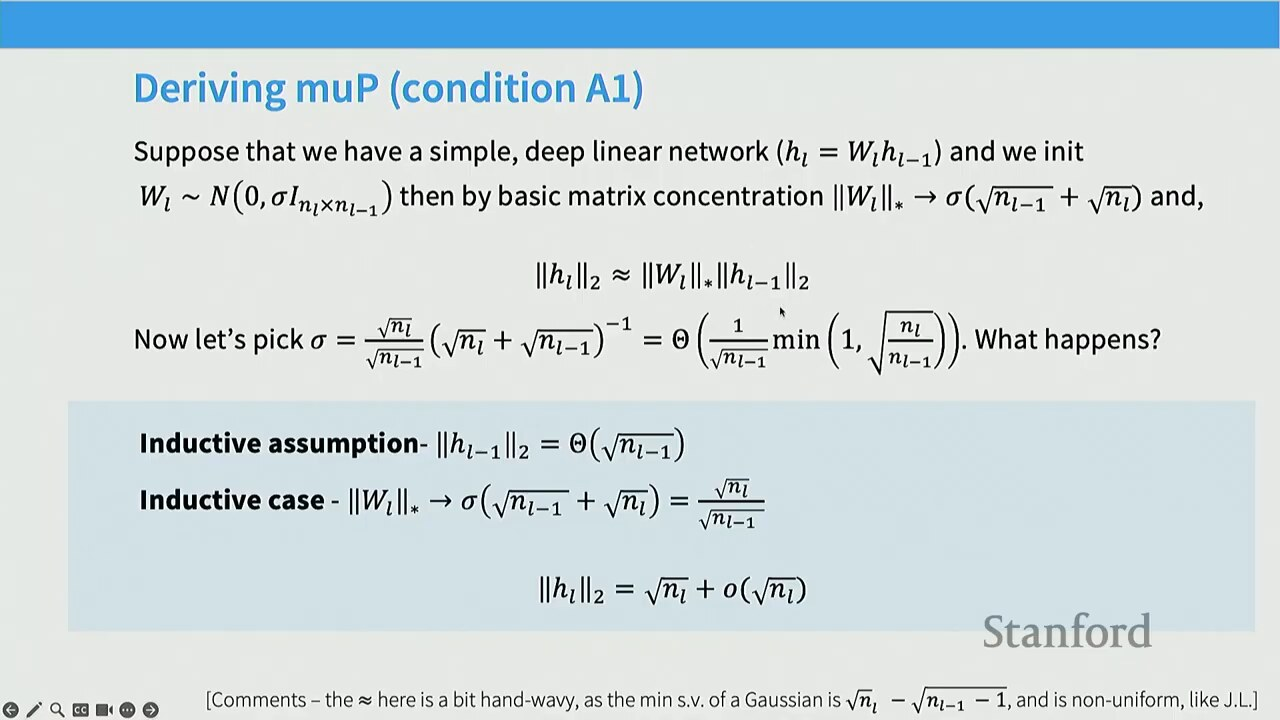
\includegraphics[width=\textwidth]{figures/fig_21.jpg}
\caption{Maximal Update Parametrization (µP)：理论框架的动机\protect\footnotemark}
\end{figure}
\footnotetext{视频画面时间区间：00:55:00--00:55:30。}

前面的实验观察 $\eta^* \propto 1/m$ 是经验性的。Yang et al. (2021) 的 µP 论文给出了一个\textbf{原则性}的理论框架，不仅能解释这个观察，还能推导出所有超参数（初始化方差、学习率、权重衰减等）的缩放律。

µP 的核心思想：设计一种参数化方式，使得\textbf{网络在任意宽度下，单步权重更新的"典型幅度"保持不变}。"Maximal Update"之名由此而来——它最大化但不发散。

\subsection{激活值与梯度的尺度分析}

\begin{figure}[H]
\centering
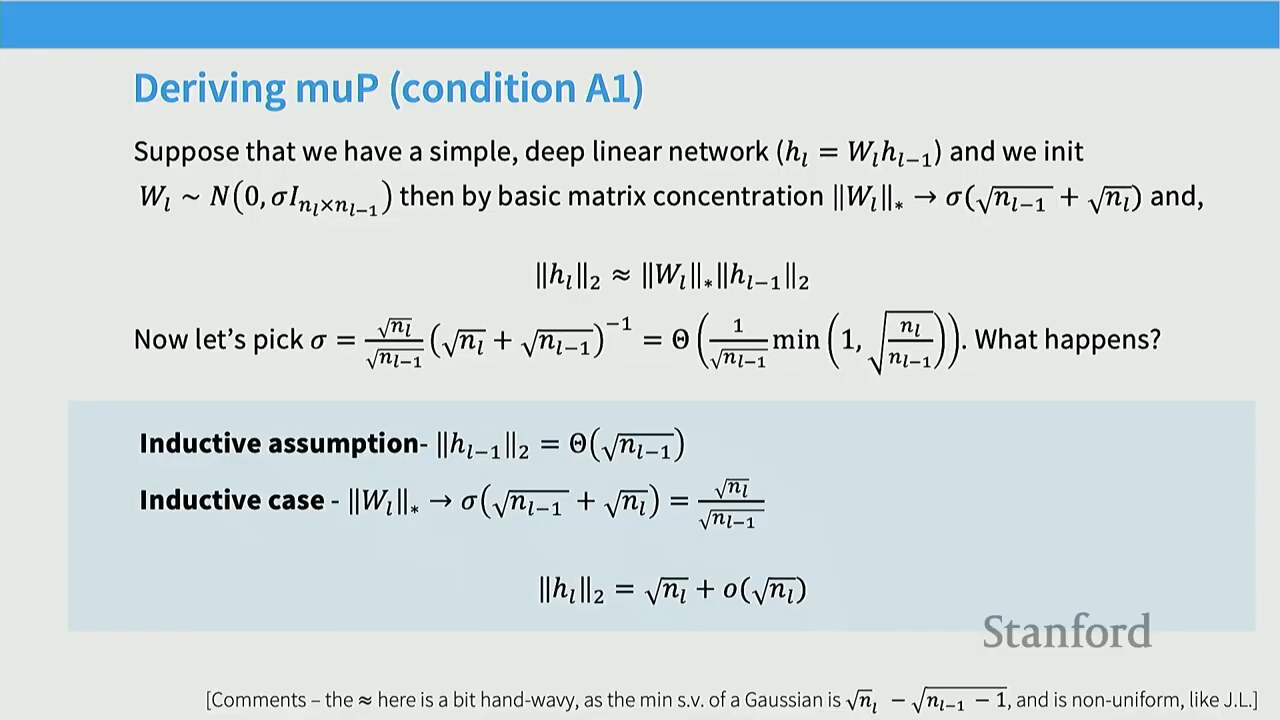
\includegraphics[width=\textwidth]{figures/fig_22.jpg}
\caption{µP：激活非消散条件——前向传播中激活的尺度分析\protect\footnotemark}
\end{figure}
\footnotetext{视频画面时间区间：00:57:30--00:58:00。}

µP 的推导从分析\textbf{前向传播}中激活值的尺度开始。考虑一个宽度为 $m$ 的全连接层：

\[
h_j^{(l+1)} = \phi\left(\sum_{i=1}^{m} W_{ji}^{(l)} h_i^{(l)}\right)
\]

\begin{itemize}
\item $h_j^{(l+1)}$：第 $l+1$ 层第 $j$ 个神经元的激活
\item $W_{ji}^{(l)}$：连接第 $l$ 层第 $i$ 个神经元到第 $l+1$ 层第 $j$ 个神经元的权重
\item $\phi$：激活函数（如 ReLU）
\item $m$：宽度（输入维度）
\end{itemize}

\begin{importantbox}{非消散条件}
为使激活 $h_j^{(l+1)}$ 在任意宽度 $m$ 下保持 $O(1)$ 的尺度（既不爆炸也不消失），权重初始化的标准差必须满足：
\[
\text{std}(W^{(l)}) \propto \frac{1}{\sqrt{m}}
\]

证明思路：假设 $h_i^{(l)}$ 和 $W_{ji}^{(l)}$ 独立且均值为零，则
\[
\text{Var}\left(\sum_{i=1}^{m} W_{ji}^{(l)} h_i^{(l)}\right) = m \cdot \text{Var}(W) \cdot \text{Var}(h^{(l)})
\]
要使这个方差与 $m$ 无关（即 $O(1)$），需要 $\text{Var}(W) \propto 1/m$，即 $\text{std}(W) \propto 1/\sqrt{m}$。
\end{importantbox}

这就是经典的 \textbf{He 初始化}（或 Xavier 初始化）的数学根源。它保证了前向传播中激活的稳定性。但 µP 还要保证\textbf{反向传播}中梯度的稳定性，以及\textbf{权重更新}的稳定性。

\subsection{µP 的完整推导}

\begin{figure}[H]
\centering
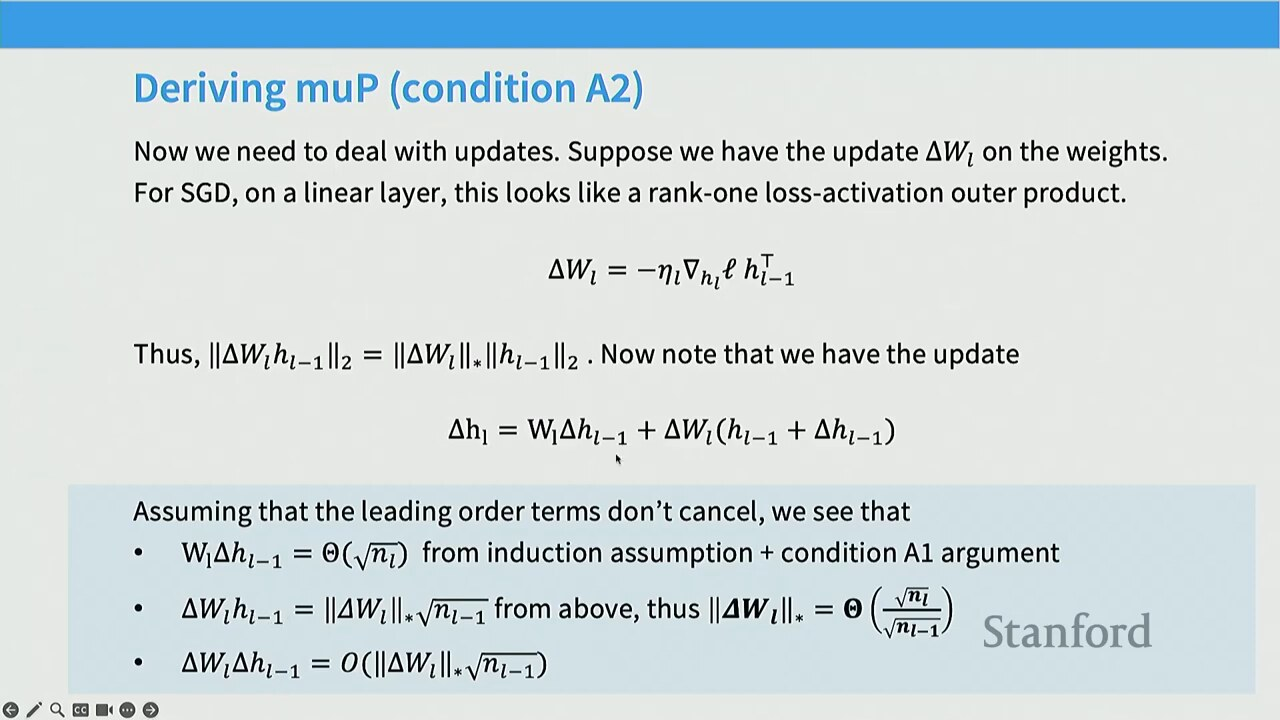
\includegraphics[width=\textwidth]{figures/fig_23.jpg}
\caption{µP：完整的数学推导——初始化、前向、反向、更新的联合尺度分析\protect\footnotemark}
\end{figure}
\footnotetext{视频画面时间区间：01:00:00--01:00:30。}

µP 的完整推导需要同时约束三个尺度：前向激活、反向梯度、权重更新。讲师给出了推导的骨架。

\begin{importantbox}{µP 的三个尺度约束}
设宽度为 $m$，权重初始化标准差为 $\sigma_w$，学习率为 $\eta$。

\textbf{约束 1（前向稳定）}：激活 $h^{(l)}$ 不随 $m$ 爆炸或消失：
\[
\sigma_w \propto \frac{1}{\sqrt{m}}
\]

\textbf{约束 2（反向稳定）}：梯度 $\partial L / \partial h^{(l)}$ 不随 $m$ 爆炸：
\[
\text{类似地，需要反向传播中梯度的方差与 } m \text{ 无关}
\]

\textbf{约束 3（更新稳定）}：权重更新 $\Delta W = -\eta \cdot \nabla W$ 的\textbf{相对幅度} $|\Delta W| / |W|$ 不随 $m$ 变化：
\[
\frac{|\Delta W|}{|W|} = \frac{\eta \cdot |\nabla W|}{|W|} = O(1)
\]

由于 $|W| \propto \sigma_w \propto 1/\sqrt{m}$，而 $|\nabla W|$ 在反向稳定下与 $m$ 无关（$O(1)$），要使比值 $O(1)$，需要：
\[
\eta \propto \frac{1}{\sqrt{m}} \cdot \frac{1}{O(1)} \cdot \sqrt{m} \quad \Rightarrow \quad \eta \propto \text{const or } 1/m
\]

具体形式取决于层的类型（输入层、隐藏层、输出层），µP 对不同层给出不同的缩放律。
\end{importantbox}

\subsection{初始化稳定性}

\begin{figure}[H]
\centering
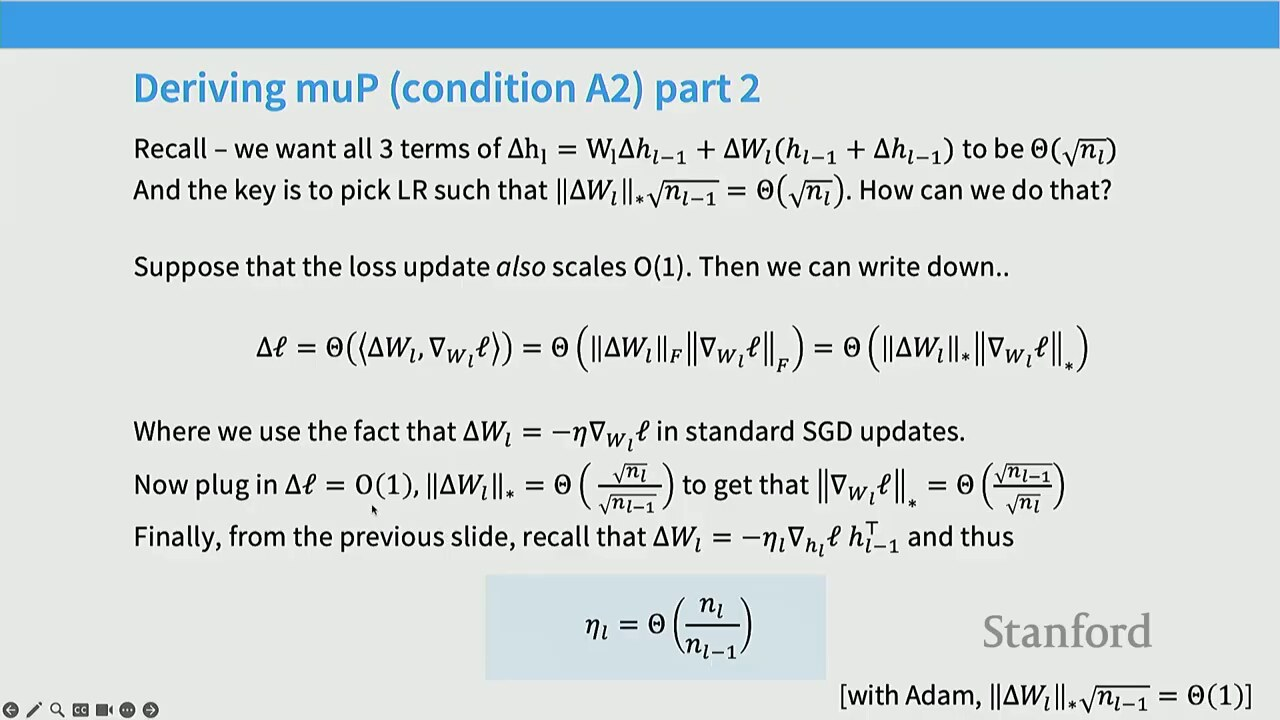
\includegraphics[width=\textwidth]{figures/fig_24.jpg}
\caption{µP：初始化稳定性——不同宽度下的初始激活分布\protect\footnotemark}
\end{figure}
\footnotetext{视频画面时间区间：01:02:30--01:03:00。}

讲师展示了实验验证：在 µP 参数化下，不同宽度的网络在\textbf{初始化时}的激活分布几乎重合（尺度都是 $O(1)$）。而在标准的 NTP（Standard Parametrization）下，宽网络的初始激活会发散或消失。

\begin{tabular}{p{4cm}p{5cm}p{4cm}}
\toprule
\textbf{参数化} & \textbf{权重初始化} & \textbf{学习率} \\
\midrule
Standard (SP/NTP) & $\sigma_w \propto 1/\sqrt{m}$ & $\eta \propto 1$（常数） \\
\textbf{µP} & $\sigma_w \propto 1/\sqrt{m}$（隐藏层） & $\eta \propto 1/m$（输出层） \\
& $\sigma_w \propto 1/m$（输出层） & $\eta \propto 1$（隐藏层） \\
NTK 参数化 & $\sigma_w \propto 1$ & $\eta \propto 1/m$ \\
\bottomrule
\end{tabular}

\vspace{0.3cm}

\begin{knowledgebox}{三种参数化的谱系}
\textbf{NTK 参数化}（Jacot et al., 2018）：无限宽极限下，网络训练等价于核回归。学习率 $\eta \propto 1/m$，使得无限宽时训练仍然有意义（否则更新太小，永远学不动）。

\textbf{Standard 参数化 (SP)}：深度学习标准做法。初始化用 He，学习率为常数。问题：宽度变化时，更新的相对幅度会变化，超参数无法迁移。

\textbf{µP}：介于两者之间。通过精心设计不同层的初始化和学习率缩放，使得有限宽度下更新幅度恒定，从而支持从小到大的超参数迁移。µP 在 $m \to \infty$ 时收敛到 NTK 极限，但在有限宽度下比 SP 更稳定。
\end{knowledgebox}

\subsection{宽度缩放推导：输出层 vs. 隐藏层}

\begin{figure}[H]
\centering
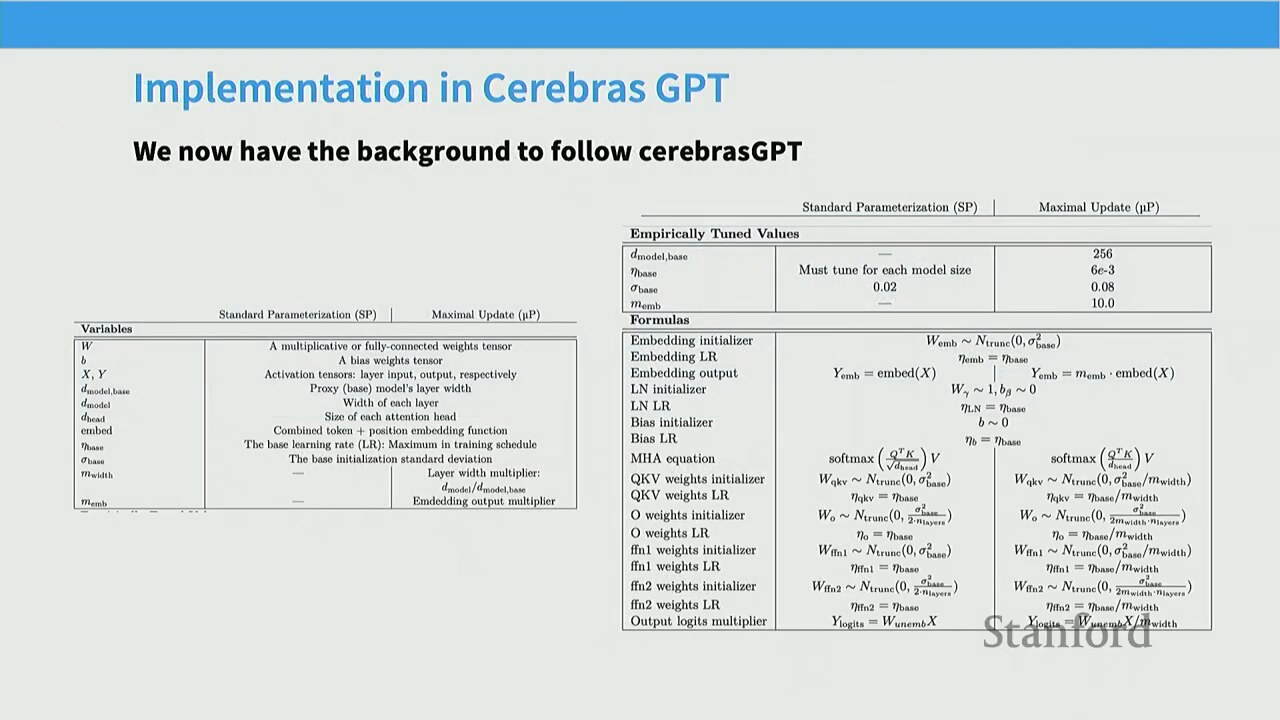
\includegraphics[width=\textwidth]{figures/fig_25.jpg}
\caption{µP：宽度缩放推导——输出层与隐藏层的差异化处理\protect\footnotemark}
\end{figure}
\footnotetext{视频画面时间区间：01:05:00--01:05:30。}

µP 的精妙之处在于它对不同层采用不同的缩放律。讲师详细推导了为什么：

\begin{importantbox}{输出层的特殊处理}
输出层（读出层，readout layer）连接最后一个隐藏层到输出。它的权重 $W_{\text{out}} \in \mathbb{R}^{1 \times m}$（假设单输出）。

\textbf{前向}：输出 $y = \sum_{i=1}^{m} W_{\text{out},i} \cdot h_i$。要使 $y$ 的尺度 $O(1)$，需要 $\text{Var}(W_{\text{out}}) \propto 1/m$，即 $\sigma_{\text{out}} \propto 1/\sqrt{m}$（与隐藏层相同）。

\textbf{但反向梯度不同}：$\partial L / \partial W_{\text{out},i} = (\partial L / \partial y) \cdot h_i$。由于 $h_i$ 是 $O(1)$，梯度也是 $O(1)$。

\textbf{更新的相对幅度}：
\[
\frac{|\Delta W_{\text{out}}|}{|W_{\text{out}}|} = \frac{\eta \cdot O(1)}{O(1/\sqrt{m})} = \eta \cdot O(\sqrt{m})
\]
要使这个比值 $O(1)$（不随 $m$ 爆炸），需要 $\eta_{\text{out}} \propto 1/\sqrt{m}$，或者更激进地，将输出层的初始化设为 $\sigma_{\text{out}} \propto 1/m$（而非 $1/\sqrt{m}$），这样：
\[
\frac{|\Delta W_{\text{out}}|}{|W_{\text{out}}|} = \frac{\eta \cdot O(1)}{O(1/m)} = \eta \cdot O(m) \quad \Rightarrow \quad \eta_{\text{out}} \propto 1/m
\]

µP 选择后者（$\sigma_{\text{out}} \propto 1/m$，$\eta_{\text{out}} \propto 1/m$），使得输出层在宽度变化时行为最稳定。
\end{importantbox}

\subsection{学习率与宽度的最终关系}

\begin{figure}[H]
\centering
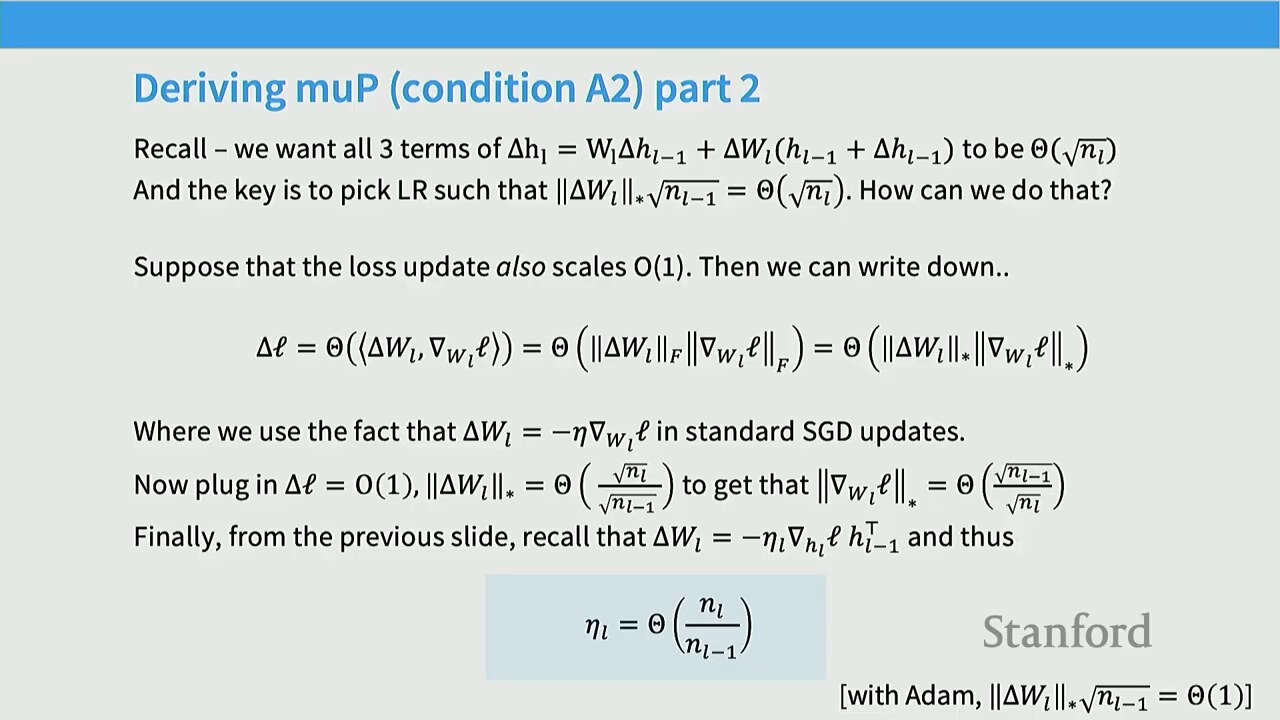
\includegraphics[width=\textwidth]{figures/fig_26.jpg}
\caption{µP：学习率 $1/m$ 关系的最终推导与验证\protect\footnotemark}
\end{figure}
\footnotetext{视频画面时间区间：01:07:30--01:08:00。}

综合所有层的分析，µP 给出的超参数缩放律为：

\begin{tabular}{p{3.5cm}p{3cm}p{3cm}p{3cm}}
\toprule
\textbf{层类型} & \textbf{权重初始化 $\sigma_w$} & \textbf{学习率 $\eta$} & \textbf{特征函数} \\
\midrule
输入层（embedding） & $1$（固定） & $1$（固定） & 无缩放 \\
隐藏层 & $1/\sqrt{m}$ & $1$（常数） & He 初始化 \\
输出层（readout） & $1/m$ & $1/m$ & 关键差异点 \\
\bottomrule
\end{tabular}

\vspace{0.3cm}

\begin{importantbox}{µP 的实践口诀}
\textbf{核心差异在输出层}：µP 把输出层的权重初始化设为 $1/m$（比标准的 $1/\sqrt{m}$ 更小），学习率也设为 $1/m$。这样，无论网络多宽，输出层的单步更新相对幅度都保持恒定。

\textbf{迁移规则}：在小模型（宽度 $m_{\text{small}}$）上搜索最优学习率 $\eta^*_{\text{small}}$，然后大模型（宽度 $m_{\text{large}}$）的学习率为：
\[
\eta^*_{\text{large}} = \eta^*_{\text{small}} \cdot \frac{m_{\text{small}}}{m_{\text{large}}}
\]

由于隐藏层学习率不随 $m$ 变（常数），只有输出层需要这个缩放。实践中，框架（如 PyTorch 的 µP 实现）会自动处理这种差异化缩放。
\end{importantbox}

\subsection{Batch size 的缩放}

µP 主要解决了学习率和初始化的迁移。Batch size 是另一个需要缩放的超参数。讲师简要提及了相关的经验规则：

\begin{itemize}
\item \textbf{临界 batch size}：存在一个 $B_{\text{crit}}$，当 batch size 低于它时，训练效率（每步进度）与 batch size 成正比；高于它时，边际收益递减。
\item \textbf{$B_{\text{crit}}$ 随训练进度增长}：训练后期，梯度方差减小，可以用更大 batch size。
\item \textbf{缩放规则}：$B_{\text{crit}}(C) \propto C$，即大计算量允许更大 batch size。
\end{itemize}

\begin{knowledgebox}{Batch size 缩放与 Chinchilla 的关系}
Chinchilla 的训练 token 数 $D$ 与 batch size $B$ 和训练步数 $S$ 的关系是 $D = B \cdot S$。如果 batch size 太小，需要更多步数（更慢）；如果太大，每步的梯度噪声不足，收敛质量下降。最优 batch size 通常取 $B_{\text{crit}}$ 的 2--4 倍，在效率和质量间取得平衡。
\end{knowledgebox}

\section{µP 的总结与实践意义}

\subsection{Summary：µP 提供了什么}

\begin{figure}[H]
\centering
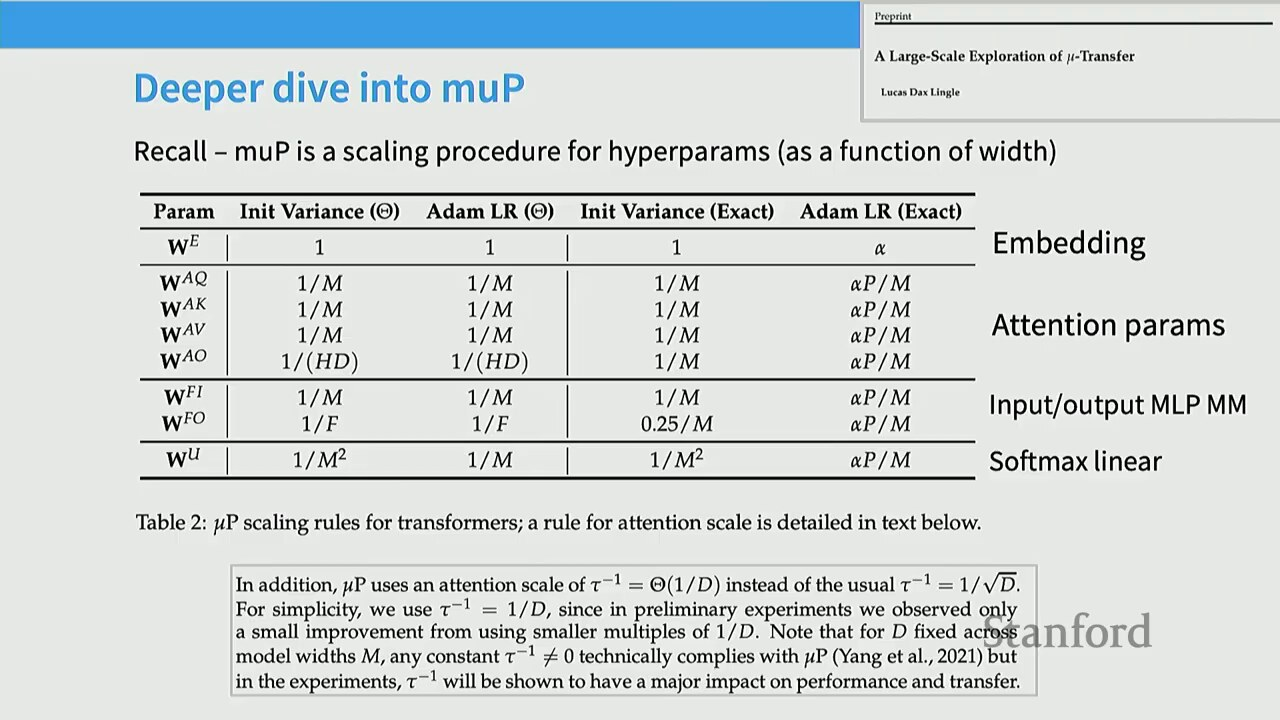
\includegraphics[width=\textwidth]{figures/fig_27.jpg}
\caption{Summary：µP 提供了原则性的超参数迁移框架\protect\footnotemark}
\end{figure}
\footnotetext{视频画面时间区间：01:10:00--01:10:30。}

\begin{importantbox}{µP 的三大贡献}
\begin{enumerate}
\item \textbf{理论统一}：µP 统一了 Standard Parametrization（有限宽度主导）和 NTK Parametrization（无限宽度极限），证明两者是连续谱的两个端点。
\item \textbf{实践迁移}：µP 使得在小模型上搜索的超参数可以直接迁移到大模型，省去昂贵的重复搜索。这是其被工业界广泛采用的主因。
\item \textbf{可解释性}：µP 揭示了"为什么大模型需要小学习率"——不是经验规律，而是激活和梯度方差随宽度增长的必然结果。
\end{enumerate}
\end{importantbox}

\subsection{µP 与 Chinchilla 的关系}

\begin{figure}[H]
\centering
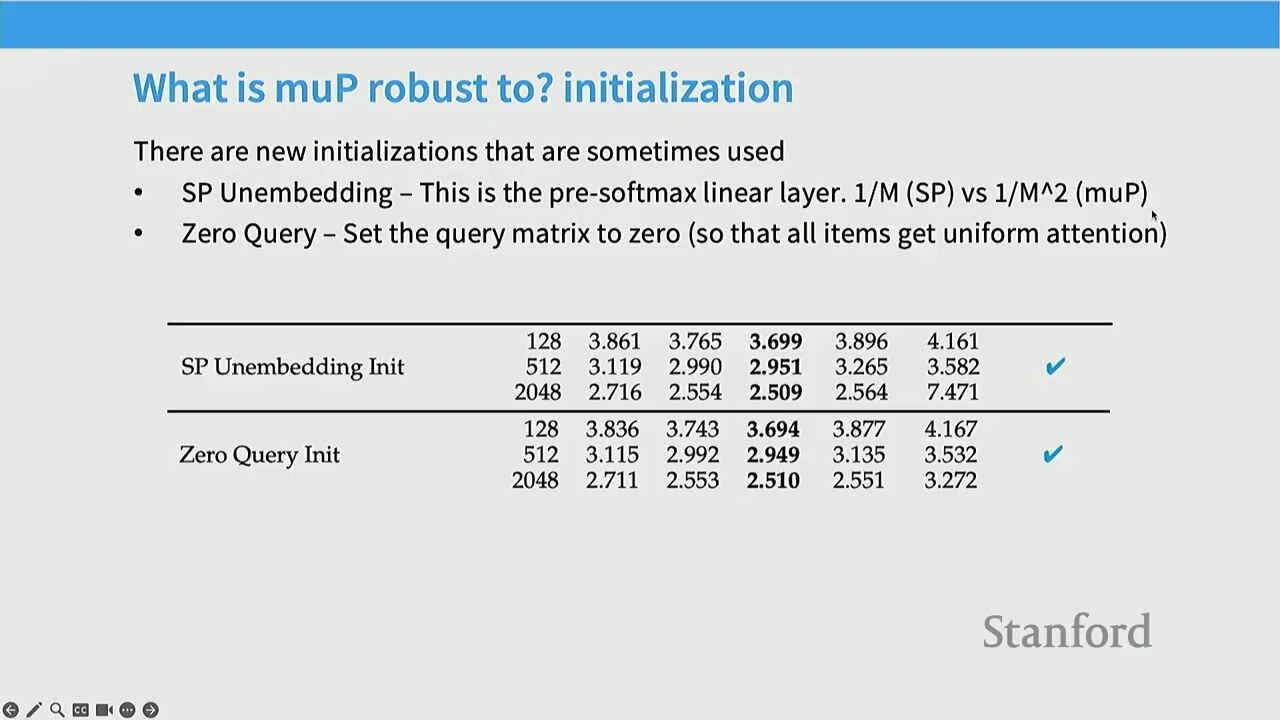
\includegraphics[width=\textwidth]{figures/fig_28.jpg}
\caption{总结与展望：µP 与 Chinchilla 的互补关系\protect\footnotemark}
\end{figure}
\footnotetext{视频画面时间区间：01:15:00--01:15:30。}

µP 和 Chinchilla 回答的是两个不同但互补的问题：

\begin{tabular}{p{3cm}p{5cm}p{5cm}}
\toprule
\textbf{维度} & \textbf{Chinchilla} & \textbf{µP} \\
\midrule
回答的问题 & 给定计算 $C$，最优 $(N^*, D^*)$？ & 给定宽度 $m$，最优超参数？ \\
关注层面 & 宏观资源分配 & 微观训练动态 \\
依赖的实验 & 多组 $(N, D)$ 训练到收敛 & 多组宽度扫描学习率 \\
产出 & 幂律指数 $\alpha$，最优比 $D^*/N^*$ & 缩放律 $\eta \propto 1/m$，$\sigma \propto 1/m$ \\
外推风险 & 极大计算量下偏差（数据耗尽） & 深度变化时需修正（µP 假设宽度主导） \\
\bottomrule
\end{tabular}

\vspace{0.3cm}

两者结合，构成了"如何训练大模型"的完整工程指南：Chinchilla 告诉你"训多大、训多少 token"，µP 告诉你"用什么学习率、怎么初始化"。

\subsection{实际模型如何偏离 Chinchilla}

\begin{warningbox}{过度训练（Over-training）趋势}
现代大模型普遍\textbf{偏离} Chinchilla 的 $D^*/N^* \approx 20$ 建议，采用更大的 $D/N$ 比：
\begin{itemize}
\item \textbf{Llama 3 8B}：80 亿参数，训练 15 万亿 token，$D/N \approx 1875$——是 Chinchilla 建议的近百倍。
\item \textbf{DeepSeek-V2}：2360 亿参数（MoE），训练 8.1 万亿 token。
\item \textbf{Qwen2.5}：0.5B 到 72B 全系，普遍过度训练。
\end{itemize}

为什么？因为 Chinchilla 只考虑\textbf{训练}计算最优，而实际部署还要考虑\textbf{推理}成本。一个小但训练充分的模型，推理更便宜。这种"inference-aware scaling"使得最优 $D/N$ 远大于 20。
\end{warningbox}

\begin{importantbox}{Inference-Aware Scaling 的逻辑}
设总成本 = 训练成本 + 推理成本。训练成本 $C_{\text{train}} \propto N \cdot D$，推理成本 $C_{\text{inference}} \propto N \cdot Q$（$Q$ 是推理查询次数）。

若 $Q$ 很大（如面向数亿用户的 API），推理成本主导，应选\textbf{更小的 $N$} 和\textbf{更大的 $D$}（过度训练），使相同性能下推理更便宜。

形式化地，最优条件变为：
\[
\min_{N, D} \left[ 6ND + \lambda \cdot N \cdot Q \right] \quad \text{s.t.} \quad L(N, D) \leq L_{\text{target}}
\]
其中 $\lambda$ 是推理的单位成本系数。解出的 $D^*/N^*$ 会随 $\lambda \cdot Q$ 增大而上升。
\end{importantbox}

\subsection{µP 的局限与开放问题}

\begin{warningbox}{µP 没有解决的问题}
\begin{enumerate}
\item \textbf{深度缩放}：µP 主要分析宽度。深度增加时，梯度消失/爆炸需要额外处理（如残差连接、LayerNorm），µP 的缩放律需要修正。
\item \textbf{非全连接结构}：Attention 层、MoE 的专家路由、稀疏结构等，µP 的标准推导不完全适用，需要针对性扩展。
\item \textbf{优化器影响}：µP 分析的是 SGD 风格的更新。Adam 等自适应优化器的缩放律更复杂，因为它们对每个参数有独立的二阶矩估计。
\item \textbf{数据依赖}：µP 假设数据分布固定。换数据集，最优超参数可能不同，µP 的迁移需要重新校准。
\end{enumerate}
\end{warningbox}

\section{总结与延伸}

\subsection{本节核心论点}

\begin{importantbox}{五个核心论点}
\begin{enumerate}
\item \textbf{Chinchilla 比 Kaplan 更可信}：通过参数化损失 $L(N,D) = E + A/N^{\alpha_N} + B/D^{\alpha_D}$ 和三种独立方法交叉验证，得出 $N^*, D^* \propto C^{0.5}$，最优 $D^*/N^* \approx 20$。GPT-3 据此被证明严重欠训练。
\item \textbf{Scaling Law 是数据依赖的统计陈述}：换数据分布，幂律指数和最优分配都会变。数据质量是最强的调节旋钮——高质量数据使最优 $D^*$ 减小。
\item \textbf{超参数迁移是独立的工程问题}：Chinchilla 不回答"学习率怎么调"。µP 填补了这个空白，从小模型推导大模型超参数，省下巨额搜索成本。
\item \textbf{µP 的核心是输出层缩放}：$\sigma_{\text{out}} \propto 1/m$，$\eta_{\text{out}} \propto 1/m$，使任意宽度下更新幅度恒定。这与 Standard Parametrization 的关键差异在输出层。
\item \textbf{实际模型偏离 Chinchilla 是理性的}：Inference-aware scaling 使最优 $D/N$ 远大于 20，因为推理成本主导，倾向于"小模型过度训练"。
\end{enumerate}
\end{importantbox}

\subsection{下节预告}

\begin{figure}[H]
\centering
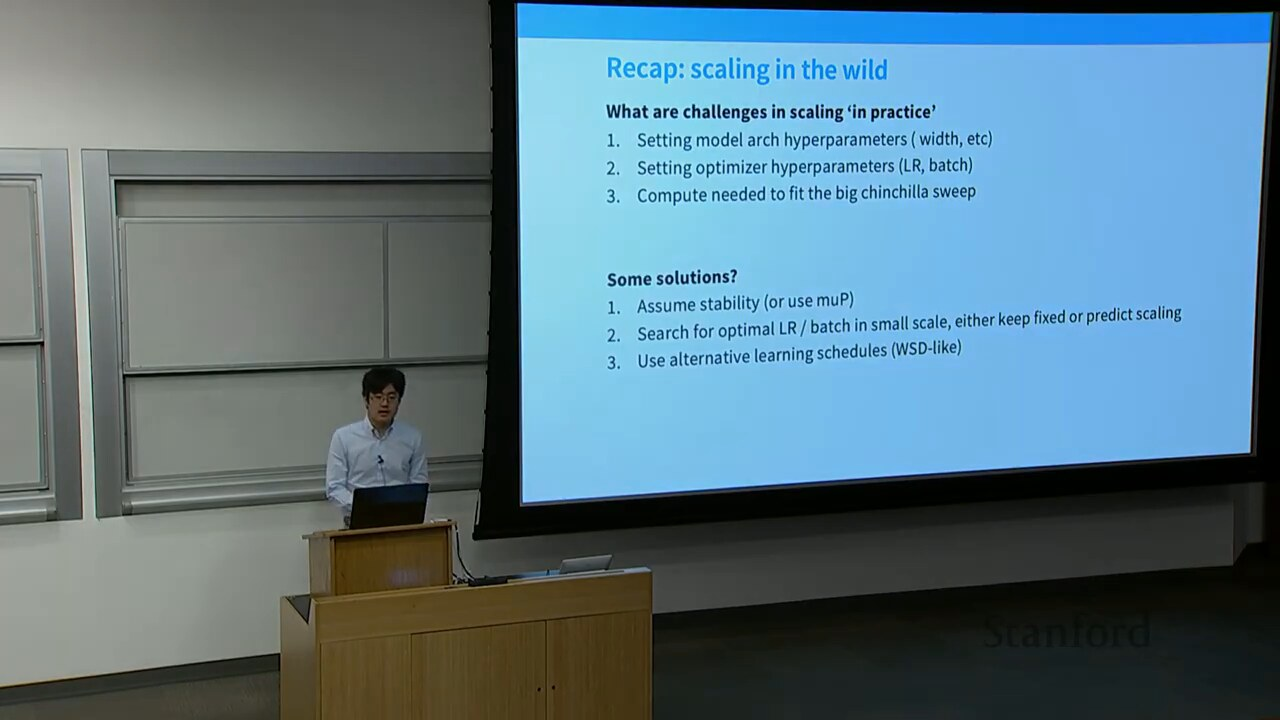
\includegraphics[width=\textwidth]{figures/fig_29.jpg}
\caption{课程结语：Scaling Laws 之后的下一步\protect\footnotemark}
\end{figure}
\footnotetext{视频画面时间区间：01:18:15--01:18:45。}

Scaling Laws 两连讲结束。后续课程将转向\textbf{数据工程}（数据过滤、去重、混合比例）和\textbf{对齐}（RLHF、DPO），这些都是在 Scaling Law 框架内提升"算法效率"的具体手段。讲师最后强调：Scaling Laws 不是终点，而是\textbf{理性分配资源的起点}——知道每个 token、每个参数的边际收益，才能做出不浪费的工程决策。

\subsection{配套阅读}

\begin{tabular}{p{8cm}p{5cm}}
\toprule
\textbf{论文} & \textbf{对应知识点} \\
\midrule
Kaplan et al. (2020) Scaling Laws for Neural LMs & Kaplan 式经验 Scaling Law \\
Hoffmann et al. (2022) Training Compute-Optimal LLMs (Chinchilla) & Chinchilla 方法论 \\
Yang et al. (2021) Tensor Programs V: Tuning Large Neural Networks via µP & µP 理论 \\
Yang \& Hu (2021) Feature Learning in Infinite-Width Networks & µP 与 NTK 的关系 \\
Hoffmann et al. -- An Empirical Analysis of Compute-Optimal LLM & 三种方法交叉验证 \\
Schaeffer et al. (2023) Are Emergent Abilities of LLMs a Mirage? & 涌现能力的争议 \\
\bottomrule
\end{tabular}

%% --- 正文内容结束 ---

\end{document}
